\documentclass[13pt]{article}
% IMPORTANT: path to the figures folder!
%\newcommand{\folder}{C:/Users/../../../figures}

%%%%%%%%%%%%%%%%%%%%%%%%%%
%% Fundamental packages %%
%%%%%%%%%%%%%%%%%%%%%%%%%%

\usepackage{siunitx} 
\sisetup{input-symbols = ()}
\usepackage{array}
\usepackage{amsmath}
\usepackage{amssymb}
\usepackage{amsthm}
\usepackage{extarrows}
\usepackage[normalem]{ulem}
\usepackage[USenglish]{babel}
\usepackage[T1]{fontenc}
\usepackage[utf8]{inputenc}
\usepackage{tgtermes}
\usepackage{ragged2e}
\usepackage{chngcntr}
\usepackage{rotating}


\usepackage{datetime}
\newdateformat{monthyeardate}{%
  \monthname[\THEMONTH] \THEYEAR} % datetime format can be changed, of course

%%%%%%%%%%%%%%
%% Geometry %%
%%%%%%%%%%%%%%

\newcommand{\linesperpagedesired}{35}
\usepackage{pdflscape}
\usepackage[left=2cm, top=2cm, right=2cm, bottom=2cm]{geometry}
\linespread{1.5}
\usepackage{changepage} % needed to make the margins of the Appendix page for additional figures a bit larger
\usepackage{adjustbox}
\usepackage{afterpage}

%%%%%%%%%%%%%%%%%%%%%%%%%%%%%%%%
%% Sections, TOC and appendix %%
%%%%%%%%%%%%%%%%%%%%%%%%%%%%%%%%
\newcommand{\secfnt}{\fontsize{14}{17}}

%\usepackage{titling}
\usepackage[compact]{titlesec}
\titleformat{\subsubsection}[runin]
  {\normalfont\largesize\bfseries}{\thesubsubsection}{1em}{}
\titleformat{\subsection}
  {\normalfont\secfnt\bfseries}{\thesubsection}{1em}{}

% if you want to change to spacing of the sections' titles use:
%\titlespacing{\subsection}{2pt}{ex}{4.5ex}

\usepackage[titles]{tocloft}
\renewcommand{\contentsname}{Table of contents}
\renewcommand{\cftsecfont}{\largefont\bfseries}% titles in bold
\renewcommand{\cftsecpagefont}{\normalfont\bfseries}% page numbers in bold

\usepackage[toc, page, title]{appendix}
\renewcommand\appendixtocname{Appendix}
\renewcommand\appendixpagename{Appendix}
 \renewcommand{\thefootnote}{\fnsymbol{footnote}}

%%%%%%%%%%%%
%% Colors %%
%%%%%%%%%%%%

\usepackage{xcolor}

\definecolor{UBonnBlue}{RGB}{0007,0082,0154}
\definecolor{Occ-A}{HTML}{EB760A}
\definecolor{Occ-B}{HTML}{43AA8D}
\definecolor{Edu}{HTML}{F9C74F}
\definecolor{Home}{HTML}{577590}

%%%%%%%%%%%%%%%%%%%%%%%%
%% Figures and tables %%
%%%%%%%%%%%%%%%%%%%%%%%%

\usepackage{booktabs}
\usepackage{longtable}
\usepackage{multirow}
\usepackage{graphicx}
\usepackage{subcaption}
\usepackage[labelfont=bf]{caption}
\usepackage{tabularx}
\usepackage{float}
\usepackage[edges]{forest}
\usepackage{tikz}
\usetikzlibrary{shapes,positioning,arrows.meta,calc,patterns}



\numberwithin{figure}{section}
\numberwithin{table}{section}
\setlength{\parindent}{0in}

%%%%%%%%%%%%%%%%%%%%%%%%%%%%%
%% Theorems and definition %%
%%%%%%%%%%%%%%%%%%%%%%%%%%%%%

\makeatletter
\newtheoremstyle{indented}
  {3pt}% space before
  {3pt}% space after
  {\addtolength{\@totalleftmargin}{3.5em}
   \addtolength{\linewidth}{-3.5em}
   \parshape 1 1.5em \linewidth \itshape}% body font
  {}% indent
  {\bfseries}% header font
  {.}% punctuation
  {.5em}% after theorem header
  {}% header specification (empty for default)
\makeatother


 {
      \theoremstyle{indented}
      \newtheorem{assumption}{Assumption}
      \newtheorem{definition}{Definition}
      \newtheorem{proposition}{Proposition}[section]
      \newtheorem{conjecture}{Conjecture}[section]
  }


\numberwithin{equation}{section} % number equations within
								 % section and subsection

\newcommand\stab[1][0.45cm]{\hspace*{4.5 mm}} % tab needed for formulas in   												  % proof in appendix

%%%%%%%%%
%% URL %%
%%%%%%%%%

\usepackage{hyperref}
\hypersetup{
	colorlinks = true,
	linkcolor = black,
	urlcolor = black,
	citecolor = UBonnBlue,
	}

%%%%%%%%%%%%%%%%%%%
%% Bibiliography %%
%%%%%%%%%%%%%%%%%%%

\usepackage{natbib}
\bibliographystyle{unsrtnat}
\renewcommand{\bibsection}{\section*{References}}
%\DeclareLanguageMapping{english}{english-apa}
%\setcounter{biburlnumpenalty}{85}
%\addbibresource{bibliography.bib} % .bib file has to be in the same directory of this file
\renewcommand{\UrlFont}{\small\ttfamily}



\title{\textbf{Research Proposal} \\ Word-of-Mouth Communication in Digital Markets}
%\fontsize{14}{14.4}\selectfont
\vspace{8ex}

\author{Iana Gerina} %\footnote{University of Vienna (VGSE),  \href{mailto:iana.gerina@univie.ac.at}{iana.gerina@univie.ac.at}}}


\begin{document}

\maketitle
\thispagestyle{empty}
%2-4 pages without bibliography

%\begin{center}
%    \textbf{Abstract}
%\end{center}

%The research proposal introduces three research ideas aimed at investigating the role of WOM communication in quality development and entry in digital markets. While the first two projects address the WOM communication effects in innovative quality development that arise in software markets, the third project investigates the consumer side of the digital product adoption and proposes that the success of penetrative pricing for a digital good highly depends on the propensity of the consumers on the market towards bargain-hunting behaviour.

%\vspace{6ex}
%\textbf{Keywords}: quality development, word-of-mouth communication, digital markets, bargain-hunting. 

\begin{center} 
\Large \textbf{Supervisors}:

\vspace{14ex}
\large Univ.-Prof. Dr. Maarten Janssen
\hspace{10ex} Univ.-Prof. Dr. Christine Zulehner

\vspace{16ex}

Vienna Graduate School of Economics

University of Vienna
\vspace{4ex}

\date{\today}
\end{center}


\clearpage
\section{Introduction} \label{motivation}
\fontsize{13.5}{14.4}\selectfont
In this research proposal I outline three projects, which are aimed at investigating the multi-faceted effects of the word-of-mouth communication on the digital markets outcomes, including product differentiation, market power and entry. This over-arching theme of the dissertation belongs to a wider branch of research on digital markets and word-of-mouth communication, and the motivation to study this particular topic is in its novelty and increasing applicability. Each year the amount of shopping online grows by 3-4\% in European countries, and the pandemic is pushing this number even higher. According to 2021 European E-Commerce Report, E-GDP of Europe has now reached 3.98\% of the total European GDP.  

With many markets being driven by word-of-mouth and reputation, all digital markets will retain an additional aspect of information exchange due to them being a part of the world-wide web. The influence of word-of-mouth communication on market outcomes, as well as the ability of the producer to optimally intervene in it has been studied extensively \citep{Mayzlin2006, Godes2009}, however, much less attention has been given to communication platforms, which by themselves allow consumers to communicate directly with each other \citep{Godes2004} and, especially, the sellers. In my first two projects I focus mainly on software development markets, which, while exhibiting many characteristics specific to them only, also allow me to gain insight into the role of collaboration, information diffusion and transparency in entrepreneurial activity and entry outside of them. My focus is the pure information diffusion effects  that arise from WOM communication and their role in software development, as opposed to the broad literature on fake reviews and the producer's manipulation of information. Thus, I am interested in the information diffusion induced market conditions that an incumbent faces and not how the producer might seek to circumvent them outside of the purchase-sell interaction. 

The main advantage of focusing on such markets is their transparency and, thus, the potential for empirical investigation. While WOM communication is commonplace in most markets, it is highly tractable in digital ones and especially digital communication platforms designed for consumer and producer communication. The mechanisms behind digital apps markets functioning continue to be a highly topical issue. Digital markets, in general, presented researchers with a number of new market formations, such as digital platforms \citep{Just2018, Choi2021, Appel2020}. Explaining the often surprising market outcomes, e.g. prevalence of zero-price markets, the coexistence of free and paid versions ("freemium"), transparency of product development despite it being a public good has long been a prevalent branch of literature \citep{Appel2020, Ajorlou2018}, as well as a vital tool for making informed policy decisions. However, my project's focus is different. I contribute to this literature by describing a different type of market interaction, enabled by digital communication. I do not investigate the role of the platforms in it, but make of its transparency and the way it mirrors the real-world interaction.

In the second section of the research proposal, I describe the first project, which focuses on the dual impact of WOM communication on the quality development decision of a start-up with an innovative idea. There are two main research questions that I address in this project: how does the communication between consumers and producers in a digital marketplace influence the investment of entrepreneurs in the quality of their goods? What is the mechanism behind WOM communication's impact on successful market entry? To better understand these effects, as well as to quantify their impact, I develop a simple theoretical model of price competition in a vertically differentiated market and use the web-scraped data from a software development forum to estimate its parameters. My intention is to disentangle the two effects from each other and provide some comparative statics that illustrate the advantages and disadvantages of the current market equilibria. 

Using the theoretical model I show that delayed diffusion of information about the new good ensures that some consumers are being kept captive by the incumbent firm, influencing market competition \citep{Fainmesser2020}, whereas from the side of supply newly attracted consumers provide additional feedback on the product's quality, making the costs of producing better quality products lower. Due to the product's development transparency, all entering firms can emulate the incumbent's good entering level of quality without any additional costs. This trade-off, I argue, results in a dual effect from the WOM communication on the market outcomes. While the pricing of the incumbent is that of the monopolist due to the demand-side effects, supply-side effects promote the good's quality development above that of a monopolist, resulting in increased welfare.

My empirical estimation, while preliminary, provides additional support to the argument. The first OLS regression of the quality development variable on the indicator of mentions of the product in external threads of the forum, showed a significant positive impact, predicted by the theoretical model. While the data collection is still in progress, I already have enough observations to describe the data set and evaluate how balanced it is, which I do in section \ref{empirics}.

%The ability of the producers to learn from their feedback is akin to the learning-by-doing effects \citet{Tirole}, as promoting higher demand in the first period results in more demand and thus, more feedback. In this way the project investigates the highly curious outcome of the digital app markets: quality development, despite the transparency and possibility of plagiarism; as well as highlighting an additional incentive to engage in zero pricing even in highly monopolised markets, adding to the standard explanation of zero marginal costs of production \citep{Ajorlou2018, Campbell2015}. In contrast to most classic learning-by-doing and knowledge spillovers literature \citep{Tirole,  Jovanovic1994}, I show that investment in quality is not hindered by learning-by-doing externality due to higher customer base effect (similar to \citet{Jovanovic1994}) and feedback effect.


In the third section of the proposal, I present the second research idea that takes a more theoretical approach to the general topic of the connection between WOM and quality development. Expanding the simplistic theoretical model of the second section, I aim to better understand why would innovators find it optimal to provide a free version of their good and the role of the WOM communication in the widespread continuous development of quality of many digital goods. My idea is to show through a dynamic model how the innovation incentives of the incumbent change with the information diffusion and what factors influence that change and the overall success of the innovative venture.



% However, as I demonstrate in the first project, delayed information diffusion through WOM communication can lead to market monopolisation. The research question that I want to address with this project is: what is the underlying mechanism of succesful entry in digital markets with WOM communication? To investigate it I formulate a structural model that I will use to estimate the threshold number of consumers that a firm must attract for its entry to be successful in the long-run. Moreover, I examine how this threshold varies depending on the WOM network structure and provide counterfactuals to demonstrate that some types of WOM networks result in natural barriers to entry. 

Finally, in the fourth section of the proposal, I describe the third planned project. Building on the recent paper by \citet{Gentry2018}, I investigate the variation in the WOM influence on the success of  penetrative pricing in markets with bargain-hunting consumers. I argue that the widespread use of penetrative pricing in discounter markets can be rationalised by the prevalence of consumers in these markets towards bargain hunting behaviour.  

%\textbf{Hypothesis:} The market consists of a small number of dominant firms, who have market power, as well as a large number of fringe firms, who are price-takers. This market outcome is due to WOM being doubly advantageous to the dominant firms and restricting the growth of fringe firms, thus resulting in natural barriers to entry. However, due to software development process being transparent to everybody, it also results in higher levels of investment in quality, as long as the market is not completely disjointed.

%However, in contrast to earlier literature I argue that in such markets, where WOM is present, marginal costs of production are not only non-zero, but also negative and decreasing in the number of consumers. In combination with WOM effects on demand, I explain how these characteristics result in the  outcomes I observe in such markets. Moreover, I investigate the properties of the WOM network in software development forums and describe their role in the process of market monopolisation, as well as quality development.


%My aim is to empirically disentangle the two effects on the market outcomes: the WOM communication leading to captive consumers and the effect of feedback on quality development resulting in reduction of costs of production for the entrant. By estimating a structural model I hope to investigate the following counterfactuals: 

%\begin{enumerate}
 %   \item "but for" feedback effect, would the incumbent still be interested in increasing the quality production? 
  %  \item would different structures of WOM communication network result in different market outcomes, e.g. less monopolisation of the market or lower quality investment?
%\end{enumerate}

\setcounter{tocdepth}{2}
\addtocounter{page}{-1}


\section{WOM and Innovative Quality in Software Development Platforms}

In the past decade, the software sector has grown at twice the rate of the aggregate of all industries (S\&P Global (as of October 2021)). While most of it is produced by software corporations, the software sector has low sunk costs, inducing, as can be seen from the data, many firms to enter. Gaining profit after entry, however, is not as likely: in the preliminary data set I have collected, less than 10\% of apps stay active after 5 years since launch.  Historically, many big software corporations started as developer teams and one innovative product (e.g. Google, Facebook and even Microsoft). In light of this, investigating entrepreneurial activity in software development markets and its conditions is particularly interesting.

For software development, however, there are specific digital communication platforms that many developers are aware of and commonly use: software development forums. The most famous one, XDA forum, "founded by developers, for developers" in 2003, counts millions of unique users among its members. While there are many sections of the forum, almost all of them have a subsection dedicated to developing software for specific device or operating system, where anyone can post either their independently developed software or request help with some software glitch or problem. The products offered in this forum are often extremely niche, catering to the needs of the audience, and range from fully developed software to a few lines of code packaged for download. By the rule of the platform, the apps must be "non-commercial", which translates to a requirement that any software published on the forum must have a free version available. This, however, does not preclude profit maximisation as most successful developers offer a paid version of the software for download as well, with a few developers, as can be seen in the scraped data, admitting that developing this project is now their main source of income.

Instead of looking into a limited number of markets, I can investigate the average effects for over two thousand separate software markets as they gradually develop further and attract new consumers by-stepping a common issue with empirical entry models. The complete transparency of communications in the forum allows for a degree of tractability of communication almost impossible to achieve for entrepreneurial activity in markets with non-digital goods. 

With this project, I aim to investigate the role of WOM communication and the collaboration of developers in the quality development decision of an innovative entrepreneur. Instead of focusing on the producers optimising their prices in a dynamic setting like \citet{Ajorlou2018}, who provide a framework to explain fluctuation of prices and the frequent zero-pricing, I focus on the market where the zero-pricing is much too pervasive to be a short-run decision, but rather a reaction to the state of the incumbent and her ability to invest in development. In this way the model allows to simply, but efficiently aggregate the effects in the market by using a small number of parameters of interest.

The idea that WOM communication is a driver behind new a product's adoption was proven to be true by \citet{Hill2006}, who showed that being connected to somebody who has adopted the service makes a consumer 3-5 times more likely to adopt it herself. WOM communication as a driver for product quality has been examined in \citet{Godes2017}. The paper in question predicts a different optimal product-policy response to the growth in social interactions between consumers, depending on whether the structure of the network changes or if it only expands. Building on these results, I aim to investigate the impact of the combination of the feedback effect and the motives behind WOM communication on the quality development decision. I not only quantify these effects for the software development markets but also explore the drivers behind the consumers' decision to share information and how this decision impacts the development of software quality.










\subsection{Fundamentals of the Model} \label{model}
 
In this subsection I set up a simple two-period game between incumbent and entrant and explain the intuition behind the model assumptions.

\textbf{Supply}:
There a 2 firms producing vertically differentiated goods following  \citet{Tirole}. However, one firm, the incumbent, enters the market earlier. In this model I am mostly interested in the optimal decisions of the incumbent, and the entrant's role is greatly simplified to reflect the threat of copying on the market. There is a base quality $s_0$, which is inherent to any innovative, working good. To increase the quality above that the incumbent can engage in costly quality production, which is a function of invested hours of work: $s=\sqrt{h +\varepsilon}$, where $\sqrt{\varepsilon} = s_0$. Moreover, the quality accumulates over periods, i.e. $s_{t+1}=s_{t}+\Delta s_t$ and $t \in \{1,2\}$. 

An important assumption here is that there is a linearly separable fixed cost $FC_t$ that an incumbent that engages in quality production must pay in every period she does so. The fixed cost is known to the incumbent. Moreover, the cost of producing quality is decreasing in the number of consumers the product was sold to in the previous period. As the incumbent introduces an innovative product, there is no feedback effect in the first period and her costs are simply $c_1= w_1h_1 + FC_1$, where $h_1$ is the number of hours the incumbent allocates to the production of the good's quality and $w_1$ is the wage of an exogenous work opportunity of the incumbent (e.g. office job). 

After the first period, however, the incumbent's cost is: $c_2= w_2h_2 + FC_2 - \alpha d_1$, where $d_1$ is the demand for incumbent's good in the first period and $0\leq \alpha \leq w$. Note that the marginal cost of producing a unit of good is 0, similar to other papers in the literature \citep{Ajorlou2018}. 

Whereas the incumbent is free to choose her hours of work and thus, quality, the entrant is only capable of copying, as there is full transparency of software development. If the incumbent has developed quality in the first period, the entrant can copy that quality fully and without cost.

\textbf{Demand}: 
Consumers derive utility from the quality of the product. Thus, each consumer's utility: $u = \theta s_t - p_{ti}$, where $\theta$ - is drawn separately and independently from $U[0,1]$ and signifies the taste of quality and $i$ corresponds to the incumbent or entrant. The outside option has a value of 0, thus, the participation constraint is $s_t \theta \geq 0$.  Each consumer only needs one good in each period and is perfectly myopic.
%The marginal consumer $\hat{j}$ is indifferent between the goods of the entrants and the incumbent, so $(s+s_0) \theta_{\hat{j}} - p = s_{i^{-inc}} \theta_{\hat{j}} - p_{i^{-inc}}$. 

%Integrating over these conditions I derive that the demand for entrant's good by consumer $j$ is: $\tfrac{ps^e - p_es}{s^e(s-s^e)}$, and the demand for the incumbent's good: $ 1 - \tfrac{p - p^e}{s - s^e}$. 

In the first period of the game, $M$ consumers are active on the market. These $M$ consumers are connected through social network to $N$ other consumers, whom they inform about the goods. Therefore, there is altogether $M(N+1)$ consumers on the market.

\textbf{Structure of the game:}
The game occurs in two periods. Initially no consumers are informed about the producers' goods. By the rules of the platform each producer must offer a free, working good. On top of that, the producers might decide to develop quality and offer a paid good.  In \textbf{$t=1$} incumbent decides whether to invest some amount of hours into developing quality, resulting in $s_1 = s_0+\Delta s_1$. She then enters the market and sets the price for this good as $p_1$. $M$ consumers become informed about the incumbent's goods, their price and quality, and each buy one unit of the good or choose an outside option. The incumbent knows how much of the good was bought, i.e. she is aware of the realised demand $d_1$, which depends on the realisations of $\theta$. 

In \textbf{$t=2$}, the incumbent again chooses (1) whether to invest some amount of hours into producing quality or not, therefore producing a new version of the good and updating her paid good's quality. If the product is offered, the quality of the new version of the good is now  $s_2 = s_1 + \Delta s_2$. To simplify the analysis, I assume that the incumbent is interested in keeping the entrant out of the market and prefers to update the quality of her freely available good to $s_1$ (2). Optimising over her profit for this price, she sets price $p_2$ for the paid good (3), simultaneously with the entering firm's pricing decisions. The new firm, capable only of copying the incumbent's previous period quality, must offer a free good, and can offer a second one with quality $\Delta s_1$. The initial $M$ consumers become informed about the entrant's good, its price and quality. Moreover, as there is a free version of the product available, all $M$ consumers try the incumbent's good and inform their $N$ friends about the incumbent's existence with probability $\gamma$, so that these newly attracted $d_1N$ consumers become informed about the goods offered by the incumbent, their prices and quality.

The initially informed $M$ consumers can buy the first-period good again (i.e. pay the next month/year subscription for using it), try the new version of the good or switch to the entrant's goods. This is in contrast with $d_1N$ newly informed consumers, who only have access to incumbent's goods and are, thus, captive.


\textbf{Intuition behind the model assumptions:} The model mirrors the development process in the market quite closely. Most importantly, software published on the forum is never deleted from it, i.e. the previous versions of the good are always available for consumers. The development process continues in stages, and the producers, who decide to switch to the "freemium" model mentioned in \ref{motivation}, as can be seen from the data, introduce a paid version of the good, while keeping the previous good available. I will explore how this decision may be optimal in the presence of the entrant(s) and her plagiarism in the second project.

The assumptions on the market structure are strongly supported by the data. While there are cases where there is more than one entering firm, the vertical differentiation of the goods implies lack of their impact on incumbent decision-making. Moreover, intuitively I define the markets for each separate software good to be very strictly bounded to the specific problem, to which they provide the solution. The goods are perfect substitutes aside from the difference in quality; in reality, there are, of course, some more general apps, that have alternatives; I intend to control for that in the estimation. 

Furthermore, it seems realistic to assume that the same set of consumers become exogenously informed first about the incumbent's good. In the context of software development forum it could mean consumers who read forum digests and check new publications in the forum regularly. I follow \citet{Campbell2013} in assuming that the consumers talk about the good only if they have bought it themselves. While this assumption may not be strictly true in reality, it provides an intuitive benchmark on how the WOM happens: it is true that people talk more about cheaper goods and high quality goods. In contrast to baseline assumptions of \citet{Campbell2013}, I do not assume that the consumers always recommend the good, if they try it, by introducing the variable of $\gamma$, which is the probability of sharing infromation.


\begin{figure}
\centering
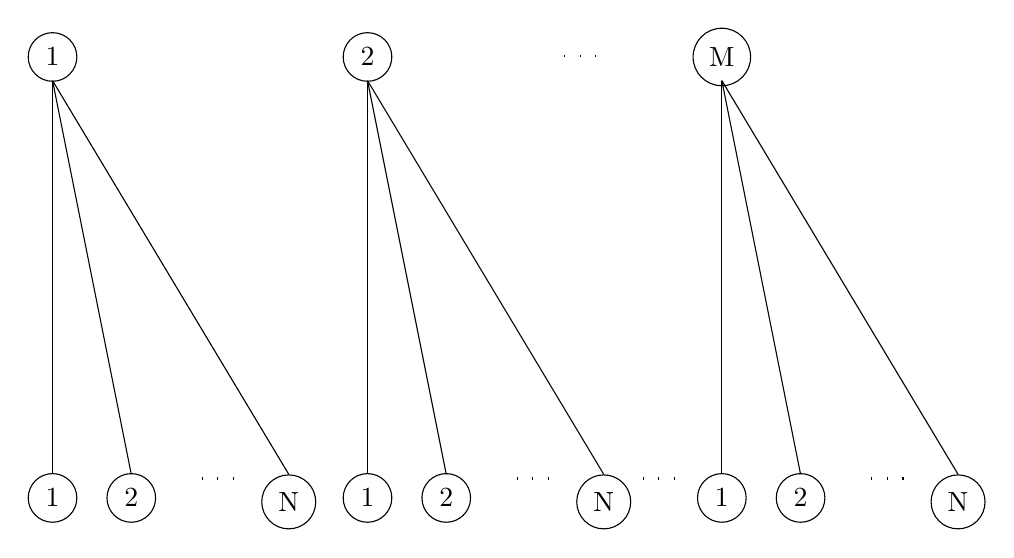
\begin{tikzpicture}
		\node[circle,draw] (c) at ((3.8, 5.3){1};
	%\draw (8.8, 5.1) circle (0.1cm) node[anchor=south] {0};
 	\draw (3.8, 5.0) -- (3.8, 0);
	\node[circle,draw] (c) at ((3.8, -0.3){1};
	%\draw (3.8, -0.1) circle (0.1cm)  node[anchor=north] {1};
 	\draw (3.8, 5.0) -- (4.8, 0);
	%\draw (5.8, -0.1) circle (0.1cm) node[anchor=north] {2};
	\node[circle,draw] (c) at ((4.8, -0.3){2};
 	\draw (3.8, 5.0) -- (6.8, 0);
	\node[circle,draw] (c) at ((6.8, -0.35){N};
	%\draw (13.8, -0.1) circle (0.1cm)  node[anchor=north] {N};
   	\draw (5.7, -2pt) -- (5.7, -1pt) ;
   	\draw (5.9, -2pt) -- (5.9, -1pt) ;
   	\draw (6.1, -2pt) -- (6.1, -1pt); 
   	
   	\node[circle,draw] (c) at ((7.8, 5.3){2};
	%\draw (8.8, 5.1) circle (0.1cm) node[anchor=south] {0};
 	\draw (7.8, 5.0) -- (7.8, 0);
	\node[circle,draw] (c) at ((7.8, -0.3){1};
	%\draw (3.8, -0.1) circle (0.1cm)  node[anchor=north] {1};
 	\draw (7.8, 5.0) -- (8.8, 0);
	%\draw (5.8, -0.1) circle (0.1cm) node[anchor=north] {2};
	\node[circle,draw] (c) at ((8.8, -0.3){2};
 	\draw (7.8, 5.0) -- (10.8, 0);
	\node[circle,draw] (c) at ((10.8, -0.35){N};
	%\draw (13.8, -0.1) circle (0.1cm)  node[anchor=north] {N};
   	\draw (9.7, -2pt) -- (9.7, -1pt) ;
   	\draw (9.9, -2pt) -- (9.9, -1pt) ;
   	\draw (10.1, -2pt) -- (10.1, -1pt); 
   	
   	\draw (11.3, -2pt) -- (11.3, -1pt) ;
   	\draw (11.5, -2pt) -- (11.5, -1pt) ;
   	\draw (11.7, -2pt) -- (11.7, -1pt); 
   	
   	\draw (10.3, 5.33) -- (10.3, 5.3) ;
   	\draw (10.5, 5.33) -- (10.5, 5.3) ;
   	\draw (10.7, 5.33) -- (10.7, 5.3); 
   	
   	\node[circle,draw] (c) at ((12.3, 5.3){M};
	%\draw (8.8, 5.1) circle (0.1cm) node[anchor=south] {0};
 	\draw (12.3, 5.0) -- (12.3, 0);
	\node[circle,draw] (c) at ((12.3, -0.3){1};
	%\draw (3.8, -0.1) circle (0.1cm)  node[anchor=north] {1};
 	\draw (12.3, 5.0) -- (13.3, 0);
	%\draw (5.8, -0.1) circle (0.1cm) node[anchor=north] {2};
	\node[circle,draw] (c) at ((13.3, -0.3){2};
 	\draw (12.3, 5.0) -- (15.3, 0);
	\node[circle,draw] (c) at ((15.3, -0.35){N};
	%\draw (13.8, -0.1) circle (0.1cm)  node[anchor=north] {N};
   	\draw (14.2, -2pt) -- (14.2, -1pt) ;
   	\draw (14.4, -2pt) -- (14.4, -1pt) ;
   	\draw (14.6, -2pt) -- (14.6, -1pt); 
\end{tikzpicture}
\caption{Consumers on the market}
\label{network}
\end{figure}

\subsection{Equilibria and Intuition Behind Results} \label{results}

In setting up the theoretical model I aim to investigate first and foremost two separate effects, which reflect the WOM influence on the market. Not unlike learning-by-doing effects in \citet{Tirole}, I assume that investments in quality become less costly with the number of attracted consumers. This reflects one of the main features of software development markets, as the product is often discussed openly among developers, who are likely to report 'bugs' directly to the producer. The parameter $\alpha$ corresponds to such an effect. 
 
Secondly, I am interested in the effect of delayed diffusion of information about goods on the market outcomes. I first look at the effect of the variables $N$ and $\gamma$, which correspond to the number of consumers that each consumer can inform and the probability that information reaches them. In the baseline model this parameter enters with a coefficient $\gamma$, which implies that the effect of information diffusion is the same among all products. In the empirical part I check if this assumption holds by introducing a number of exogenous variables that could affect $\gamma$.

Following \citet{Tirole} and denoting $\tilde{\theta}$ as the taste parameter of a consumer, who is indifferent between two goods, the demand for two differentiated goods with $s_1 \leq s_2$ on the markets can be described as follows: 
$$Prob(\theta \leq \hat{\theta}) = \tilde{\theta} - \tfrac{p_1}{s_1} = \tfrac{p_2-p_1}{\Delta s} - \tfrac{p_1}{s_1} = \tfrac{p_2s_1 - p_1s_2}{s_1\Delta s}$$ 
$$Prob(\theta \geq \tilde{\theta}) = 1 - \tilde{\theta} = 1 - \tfrac{p_2-p_1}{\Delta s} = 1 - \tfrac{p_2 - p_1}{\Delta s}$$
      
Intuitively, when there is no difference in quality between two goods, the competition is in price. For a monopolist-producer, who is forced to provide a free version of her good and offering a paid version of the good with $p_1$ and $s_1 = s_0 + \Delta$ the demand is $d_1 = 1 - \tfrac{p_2}{\Delta s_1}$, i.e. the demand the incumbent faces in the first period. In the absence of another firm's entry and information diffusion effects the incumbent would not have any incentive to increase her quality, as her optimal price and quality were already chosen to optimise her profit. The entry of another firm, which copies the incumbent's first-period quality, and the influx of new $d_1N$ consumers in the second period, results in the incumbent offering a higher quality good for free and the overall increase of the consumer welfare, as the form of profit maximisation problem remains unchanged, aside from the reference point of quality development, which is now pushed from $s_0$ to $s_1$. I investigate the incentive for the incumbent to update his free version of the good more deeply in the section 3 of the proposal.


Starting from \textbf{second period}, building on the assumption that the incumbent prefers to set the free good's quality to $\delta s_1$ and thus deter entry, I argue that the entrant then will be forced to only offer a free good of quality $\Delta s_1$ as she can not develop any quality of her own and is forced to compete over the $M$ initially informed consumers in price. 
The maximisation problem of the incumbent is as follows:
$$
\begin{aligned}
\max_{p_2,s_2} \quad &  M(1+\gamma N)(1-\tfrac{p_2}{\Delta s_2})p_2 - w_2\Delta s_2^2 - FC_2\\
\textrm{s.t.} \quad &p_2 \geq 0\\
\end{aligned}
$$



\begin{proposition}
The incumbent decides to invest in quality development in the second period if her fixed cost of development is below her profit from producing optimal amount of quality and the benefit from receiving feedback from the previous period's consumers:
$FC_2 \leq \tfrac{M^2(1+\gamma N)}{64w_2} + \alpha Mw_1$
\end{proposition}

When the proposition 1 is not satisfied, the incumbent prefers not to invest in quality, and thus, can not offer a paid version of the good, as her previous period's good quality she now offers as a free good to deter the entrant. Her profit in this case is simply the benefit from receiving feedback $\alpha w_1 M$. The profit from producing a good of optimal quality is then always below 0, and thus, always below $\alpha w_1 M$.

\begin{proposition}
In the second period of the game the level of quality development of innovative incumbent, if she decides to produce quality, depends positively on average number of friends each consumer informs ($N$) and the probability of them doing so ($\gamma$) and the pool of initially informed consumers ($M$) and negatively on her costs ($w$) in the following way:
$$\Delta s_2 = \tfrac{M(1+\gamma N)}{8w_2}$$
\end{proposition}

These results are the interior solution of the incumbent's constrained profit maximisation problem.
As in either case the second period profit of the incumbent does not depend on her first period strategy, the optimal price and quality in the first period do not depend on the state. Then by backwards induction and denoting $\pi_2^{k}$ where $k \in {1,2}$ are the two possible states in the second period, in the \textbf{first period} the incumbent's profit maximisation problem is:

$$
\begin{aligned}
\max_{p_1,s_1} \quad & Mp_1(1-\tfrac{p_1}{\Delta s_1}) - w_1 \Delta s_1^2 -FC_1 + \pi_2^{k}\\
\textrm{s.t.} \quad &p_1 \geq 0\\
\end{aligned}
$$


\begin{proposition}
In the first period the incumbent develops $\Delta s_1 = \tfrac{M}{8w}$ optimal amount of quality iff $FC_1 \leq \tfrac{M^2}{64w_1} + \beta(\tfrac{M_1^2(1+\gamma N)}{64w_1} + \alpha M_1w_0 - FC_2)$ .
\end{proposition} 

It is then possible to describe four pure strategies sub-game perfect Nash equilibria of the game. Depending on the values of $FC_1$ and $FC_2$ the incumbent either decides to develop quality in neither of the periods, one of the periods or both of them, setting the quality equal to that described in Proposition 2.2 and 2.3.

\textbf{Discussion:} The majority of model implications seem intuitive: the bigger the market, the higher the speed of information diffusion, the more incentives the producer has to develop quality. The feedback effect, on the other hand, enters the model when the decision to invest or not in quality development is made. If it's high, the probability of the incumbent developing more than a basic, free version of the good and thus, gaining profit, is higher. As the platform forces the producers to offer a free good, the information about the good diffuses as fast as it possibly can, depending on the value of $\gamma$. Moreover, even if the incumbent never develops a paid version of the good she still gets at least marginally compensated by consumer feedback, which can be alternatively interpreted as additional utility from altruistic behaviour.


\subsection{Empirical Estimation} \label{empirics}

\textbf{Empirical strategy:} The theoretical model is set up in such a way so as to simplify empirical inference. Comparing the optimal choice for quality development, if the incumbent decides to engage in it, it is clear to see that the second period equation collapses to the first period one for $N=0$. Furthermore, to make each stage truly independent of another, I relax the assumptions on $M_i$ being constant between stages (i.e. $M_{1\tau}=M_{2\tau-1}+\Delta M_{1\tau}$), which allows me to take into account the unobserved part of the information diffusion, as well as additional consumers, who become aware of the product exogenously in this stage.


\begin{figure}

\centering
\caption{Stage $\tau$}
\label{fig:time}
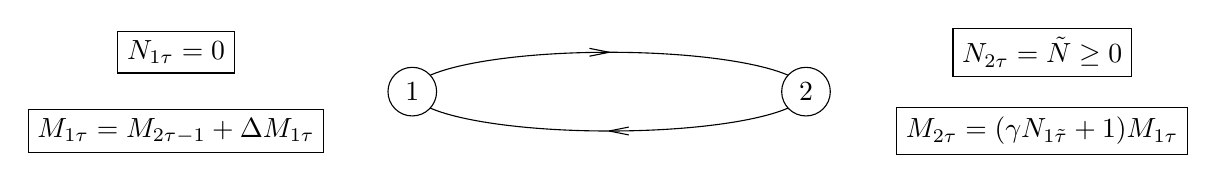
\begin{tikzpicture}
  


    \node[draw] at (2,-0.5) {$M_{1\tau}=M_{2\tau-1}+\Delta M_{1\tau}$};
    \node[draw] at (2,0.5) {$N_{1\tau}=0$};
    %\node[draw] at (1,0) {$N_{1\tau}=0$};
    %\node[draw] at (1,0) {$M_{2\tau}=\sum_{\tilde{\tau}=1}^{\mathcal{T}}M_{1\tilde{\tau}}$};
    %\node[draw] at (1,0) {$N_{1\tau}=0$};

   	\draw (10,0) arc
    [
        start angle=0,
        end angle=360,
        x radius=2.5cm,
        y radius =0.5cm
    ] ;
    \draw (7.5, 0.5) -- (7.25, 0.55);
    \draw (7.5, 0.5) -- (7.25, 0.45);
    \draw (7.5, -0.5) -- (7.75, -0.55);
    \draw (7.5, -0.5) -- (7.75, -0.45);
   	\node[circle,fill = white, draw] (c) at (10, 0){2};
   	\node[circle,fill = white,draw] (c) at (5, 0){1};
   	
    \node[draw] at (13,-0.5) {$M_{2\tau}=(\gamma N_{1\tilde{\tau}}+1)M_{1\tau}$};
    \node[draw] at (13,0.5) {$N_{2\tau}=\tilde{N}\geq 0$};
\end{tikzpicture}
\end{figure}


To better describe the timestamps of the variables I use consider Figure \ref{fig:time}. In this way I can describe the development of product in time as if occurring in each stages, where each stage $\tau \in \mathcal{T}$ is sufficiently characterized by the theoretical model. The incumbent starts the stage with some accumulated demand. She sells her product to the accumulated consumers, and the formula below takes that into account. In the beginning of the stage $N_{1\tau}=0$, as all the consumers attracted by the previous stages have been already included in period $M_{1\tau}$. The new $M_{2\tau}$, as well as the $N_{2\tau}$ that these new consumers will attract, are the ones that will decide the optimal quality development in this stage. At the end of the stage, these consumers are summed together into a $M_{1\tau+1}$. Assuming I observe the $M_{2\tau}$ for any period $\tau \in \mathcal{T}$, the baseline empirical equation for quality development can be written as:

\begin{equation}
f(\cdot) = \Delta s_{i\tau} = \tfrac{M_{i0\tau}(1+ \gamma_{i\tau} N_{i\tau})}{8w_{i\tau}(\phi)} = \tfrac{M_{i0\tau} +\lambda( \gamma_{i\tau} M_{i1\tau-1}N_{i1\tau} + \gamma_{i\tau}\Delta M_{i0\tau}N_{i1\tau})}{8w_{i\tau}(\phi)}
\end{equation}

This allows me to separate the effects from two parts of the demand: the customer base and the consumers those customers inform. The index $i$ denotes each company in the data and $\tau$ a stage of each observation. Each observation has a timestamp 0 and a timestamp 1. As I do not perceive the real cost of an hour of effort, I use a number of proxies \textbf{$w_x^j$} in a $w_{i\tau}(\phi)$ function, where $\phi$ is a vector of parameters with which these proxies enter the equation. By assumption, the wage costs do not necessarily differ within one stage. While the values of parameters themselves are not of import, choosing the right variables for this estimation is vital for future inference. I use a number of exogenous parameters to check for robustness of results and I describe them in more detail in the data subsection below.

The parameter $\lambda$ corresponds to the effect of the WOM communication on consumer development. The theoretical model implicitly assumes that this effect is 1 and that the the probability of mentioning the good to anybody is independent of the consumer's number of friends, which very well not be the case. If this parameter is 1, then the only impact is that of a customer base growing; a parameter higher than that, however, implies some multiplier effects present, which can be the result of specific network structure or the expectation of the producer that the tractable $N$ is just a fraction of the real recommendations happening outside the forum. The opposing scenario, when $\lambda$ is below 1, would imply that the producer does not expect that these mentions would attract as many consumers as were informed about the good, which could also be rationalised by some forms of social network structures. I plan to estimate an additional model, where I assume that the probability of newly informed consumers receiving and following up on a recommendation varies depending on the characteristics of the developer, average characteristics of the recommenders. Moreover, to check if the probability of mentioning the good to anybody is independent of the consumer's number of friends, I plan to introduce some additional instruments to check how sensitive the results are to this assumption.

\begin{equation}
f(\cdot) = \Delta s_{i\tau} = \tfrac{M_{i0\tau} +\lambda( \gamma_{i\tau}(\psi) M_{i1\tau-1}N_{i1\tau} + \gamma_{i\tau}(\psi)\Delta M_{i0\tau}N_{i1\tau})}{8w_{i\tau}(\phi)}
\end{equation}

Finally, assuming that different mentions have different impact, I would include in the estimation a weight matrix $W_N$ and a vector $\textbf{N}_{it}$, where each mention's impact is weighted by different characteristics, which define he consumers within the sub-forum, where the product was mentioned. I am currently in the process of collecting relevant data for this part of estimation.

\begin{equation}
f(\cdot) = \Delta s_{i\tau} = \tfrac{M_{i1\tau}(1+\lambda\gamma_{i\tau} W_NN_{i1\tau})}{8w_{i\tau}(\phi)} 
\end{equation}

The equations (2.1), (2.2) and (2.3) I then plug in the main equation estimation, which describes the probability of the incumbent introducing a paid good. The theoretical model provides an intuitive and simple way of estimating this probability. Using the propositions 2 and 3 and assuming that the incumbent expects himself to behave optimally in the future and starting from any point in the lifetime of a product the incumbent will introduce a paid version of the good in stage $\tau$ if and only if her benefit from doing so is above her costs:

\begin{equation}
Pr(p_{i\tau}\geq 0) = Pr(FC_{i\tau} \leq \alpha w_{\tau}(\phi)M_{i1\tau-1 }  + M_{i2\tau}f(\cdot) + \epsilon_{i\tau}  )
\end{equation}

% + \alpha \beta M_{it+1} w_{it}(\phi)

Thus, at any stage a producer has an option of switching to producing a paid good, and her expected profit from this includes the benefit of accumulated feedback and the profit from producing a good of optimal quality in this stage. Estimating this equation using equations (2.1), (2.2) and (2.3) I am interested in the parameters $\alpha$, \textbf{$\psi$} and $\lambda$. Their signs and magnitude reveal the role of WOM communication and feedback in quality development decision. While the $\lambda$ parameter estimation follows directly from FOC of the model, the main complexity arises when estimating parameter $\alpha$, which corresponds to the impact of consumer feedback. Separating these two effects, especially since they both depend on $M$, number of informed consumers each period, is non-trivial, and I am currently revising the estimation strategy to ensure that it provides a way to do so. 

The main issue with the estimation strategy is the endogeneity concern. While the model assumes that the the quality and the price of the product depend on exogeneous variable $M$, I do not perceive this variable in practice, but only the demand, which is accumulated through periods and must depend on price. As the quality depends on accumulated demand and demand on accumulated quality, some instrument variables are needed to avoid a bias both in the estimation of $\Delta s$ . Doubly so for the equation (2.5), where the probability of producing quality is determined through profit, which depends on demand and quality with opposite signs. 

I propose a number of demand instruments for this estimation. First of all, as I mentioned before, the forum is divided into subcategories for specific types of software and different devices. While I have been focusing on web-scraping pages with Android apps and their development, I can collect the prices for similar software for PC use, when available. Secondly, I could use the fact that some apps get published also in the Russian developer forum, 4PDA, which should shift the demand upwards, without affecting the quality directly. As I do not have that data available yet, the project is still a work in progress.

I intend to estimate each of the models with OLS, NLS and GNM estimators. This is still a work in progress, however, in the preliminary results subsection below I provide the results of the first OLS regression of development level, which seem to support the specification.



 
\textbf{Description of the preliminary data:} 

To collect the necessary data I have created a number of web-scrapers. The data that I have available at this moment is incomplete and most likely subject to some measurement errors, which I do my best to control for, but it allows me to do a first look at the data set that I will have at the end of the web-scraping process and check if some effects are already apparent.

The full current data set consists of 24659 product pages scraped from XDA Developers Forum and spans the time period between October 2010, when the development sub-forum has been set up, and May 2022, when I ran the scraper. However, only 5302 pages contain a link to the corresponding Google Play pages, which I need to collect the demand values for each app. This data set has been further curtailed by the necessity to collect the values of wage  proxies from previous date-stamps, which I used the WayBack Machine Archive for. Unfortunately, the Archive only collected timestamps between 2020 and 2022, which restricted the sample to only around 671 unique firms, each observed at up to 6 timestamps, which I divide into three time periods, corresponding to years 2020-2022. When multiple timestamps for a year are available, I assign the one with minimum difference between the date of XDA and Google Play timestamps. I demonstrate the distribution of unique product observations in three available years for the archived Google Play (Figure \ref{fig:dist_gp}) and XDA Developers scraped data (Figure \ref{fig:dist_xda}), as well as the full data set (Figure \ref{fig:dist_merged}), where these observations are merged with each other and the current data from both sources. 

%\begin{figure}[!ht]
%    \centering
%    \includegraphics[width=\textwidth]{baseline_pushout_comparison.png}
%    \caption{Baseline model: Comparison of inner solution and corner solution}
%    \label{fig:baseline_pushout}
%\end{figure}


\begin{figure}
\centering
\begin{minipage}{.3\textwidth}
\centering
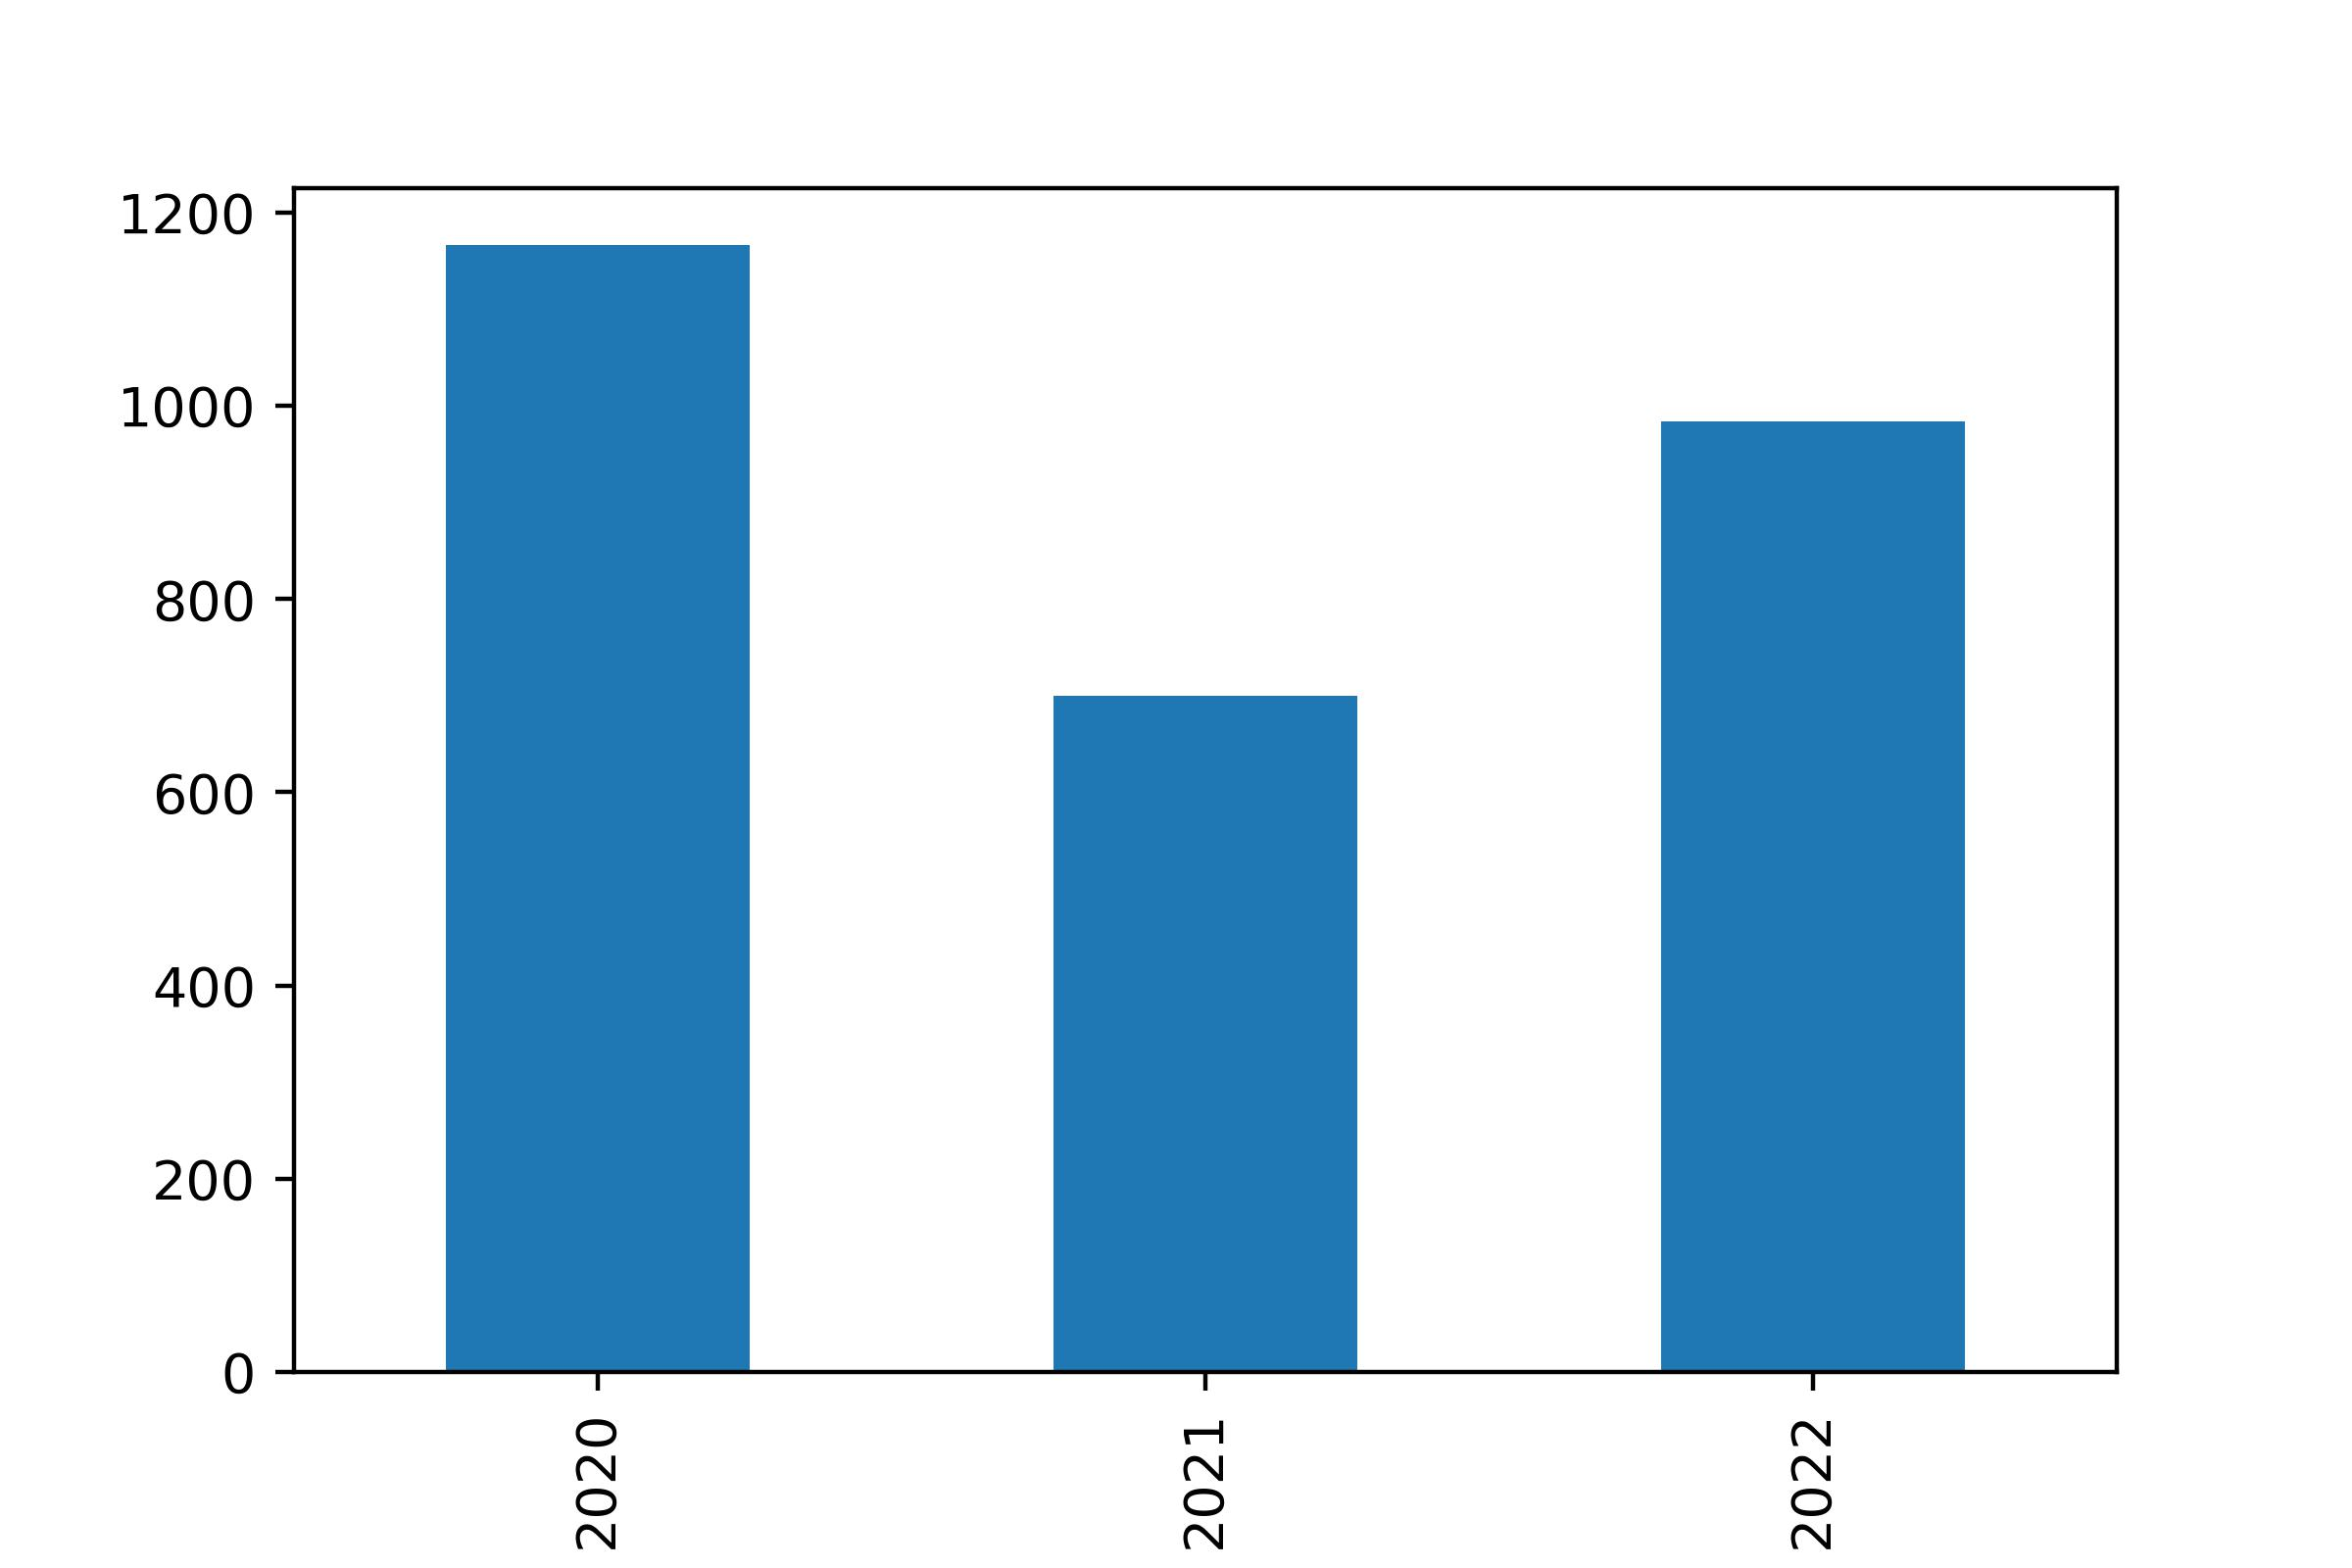
\includegraphics[width=\linewidth]{dist_gp.jpg}
\caption{Distribution of archived Google Play pages in time}
\label{fig:dist_gp}
\end{minipage}\hfill
\begin{minipage}{.3\textwidth}
\centering
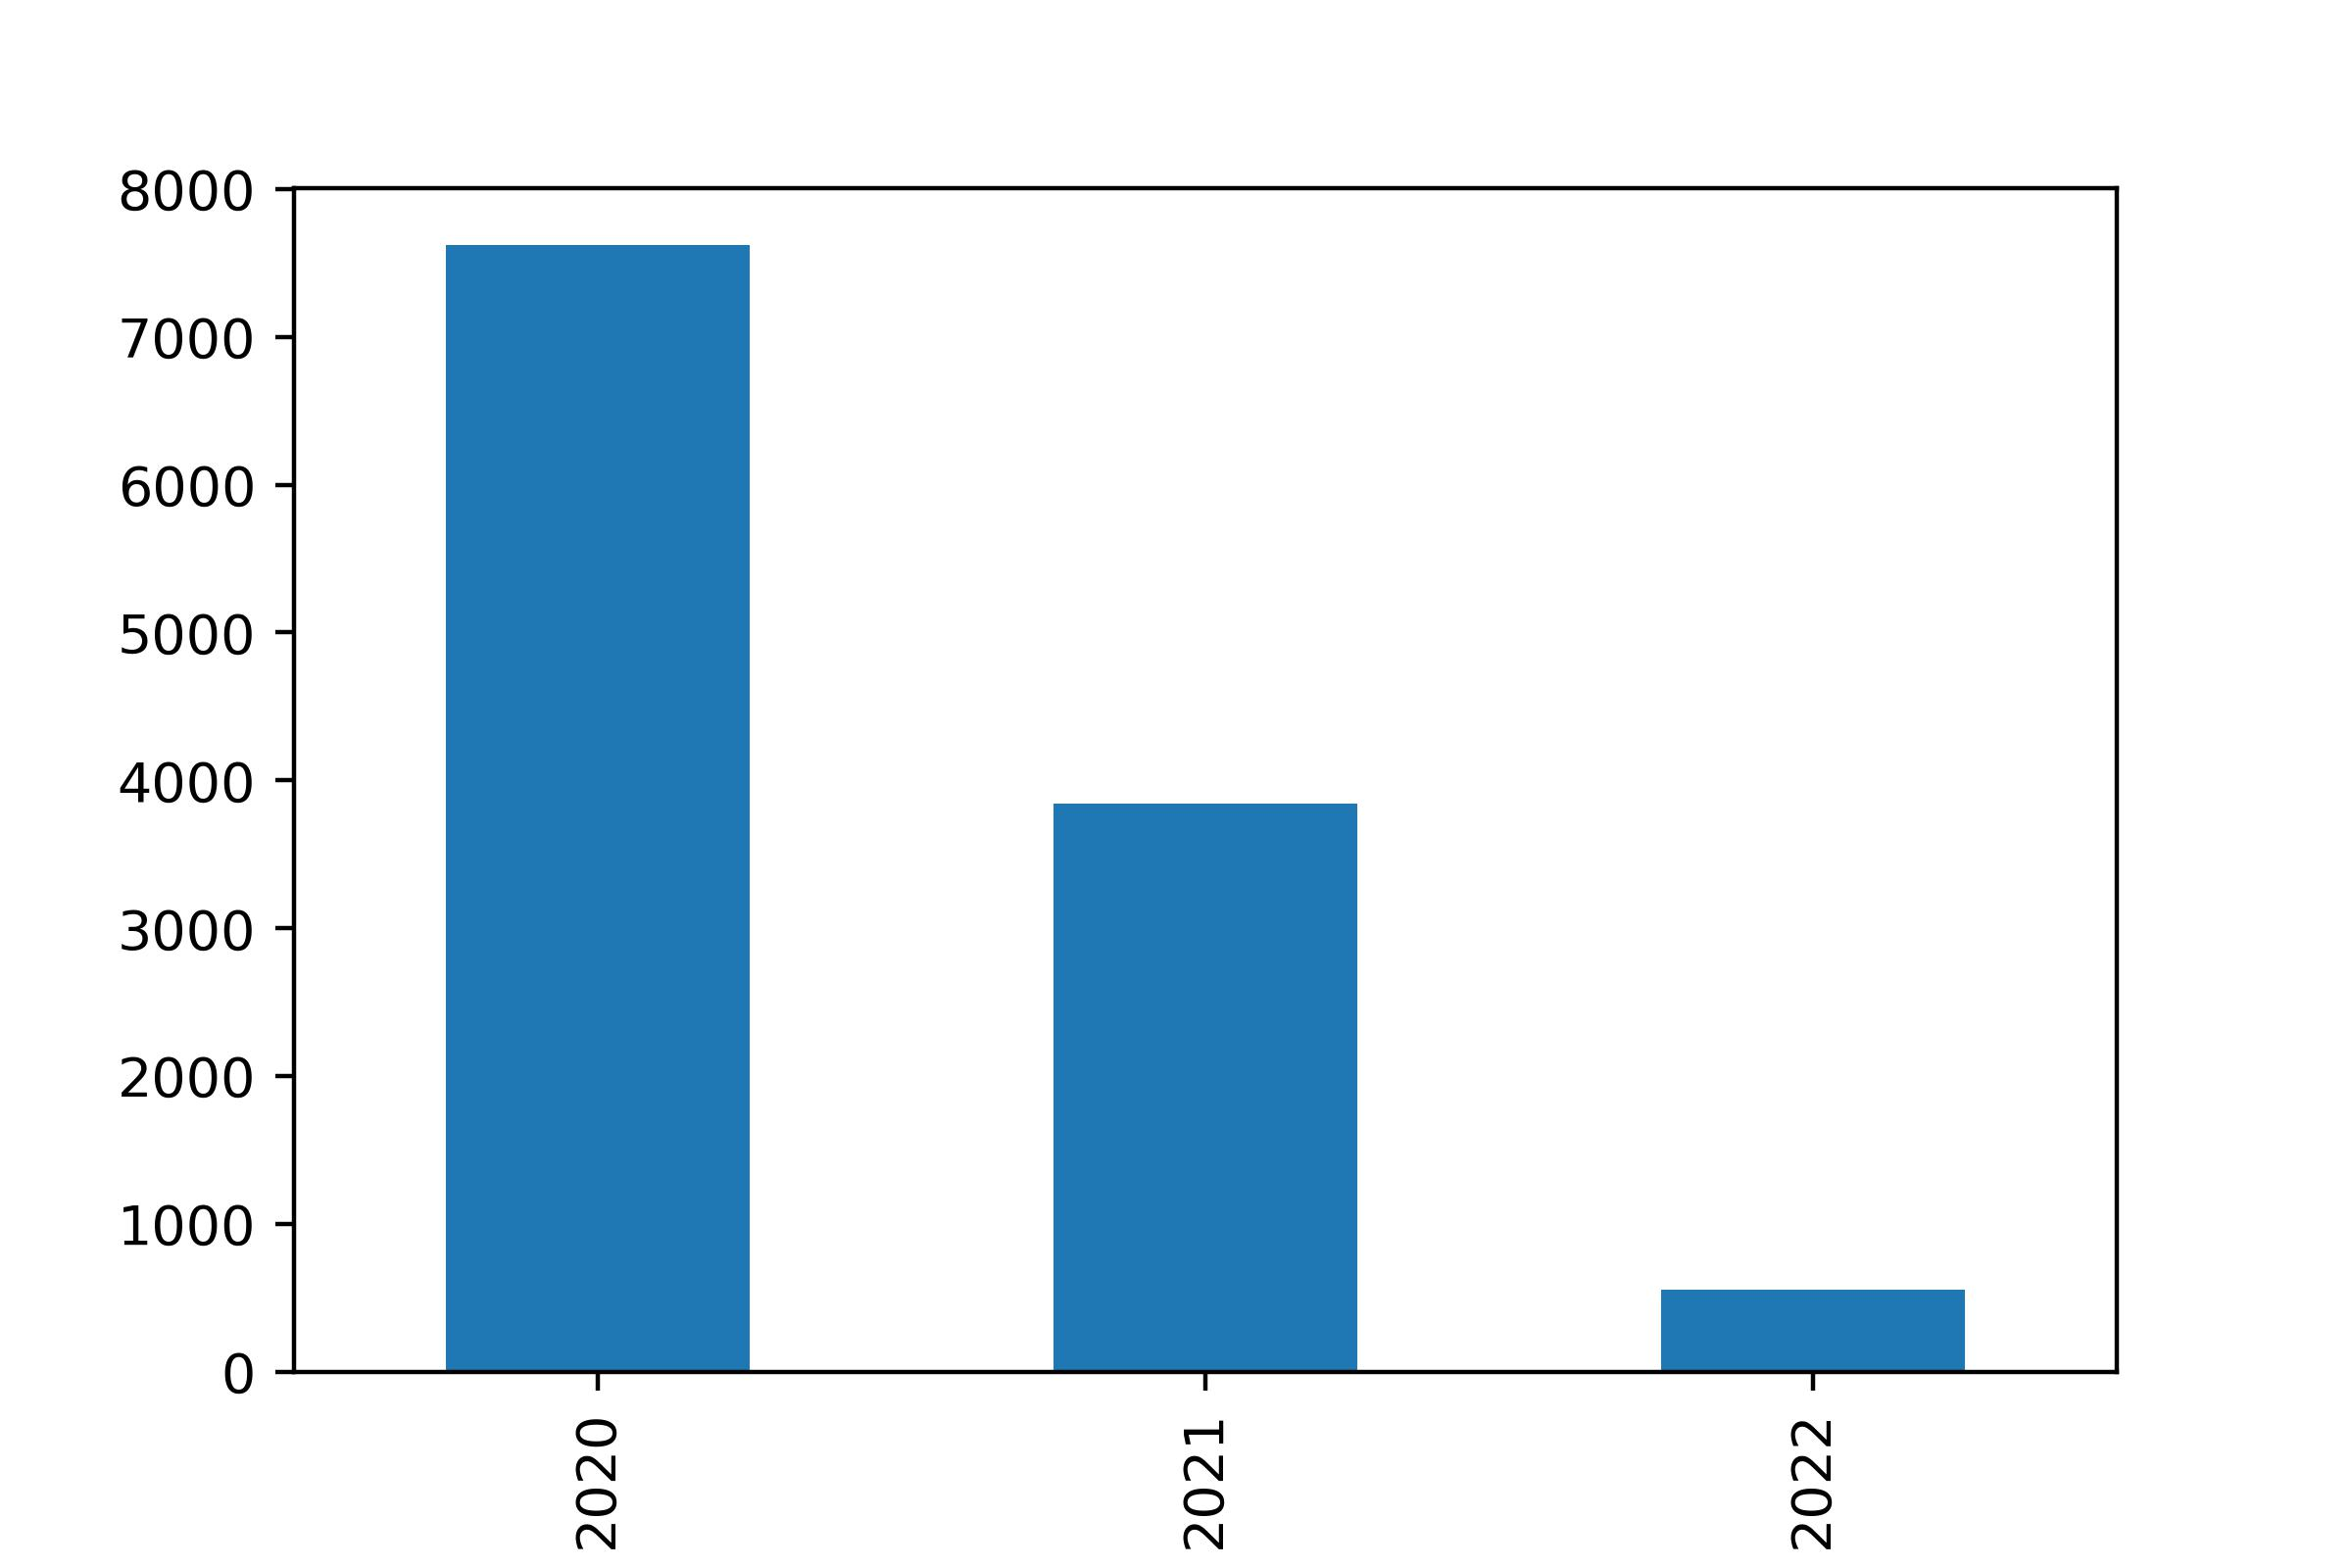
\includegraphics[width=\linewidth]{dist_xda.jpg}
\caption{Distribution of archived XDA Developers pages in time}
\label{fig:dist_xda}
\end{minipage}\hfill
\begin{minipage}{.3\textwidth}
\centering
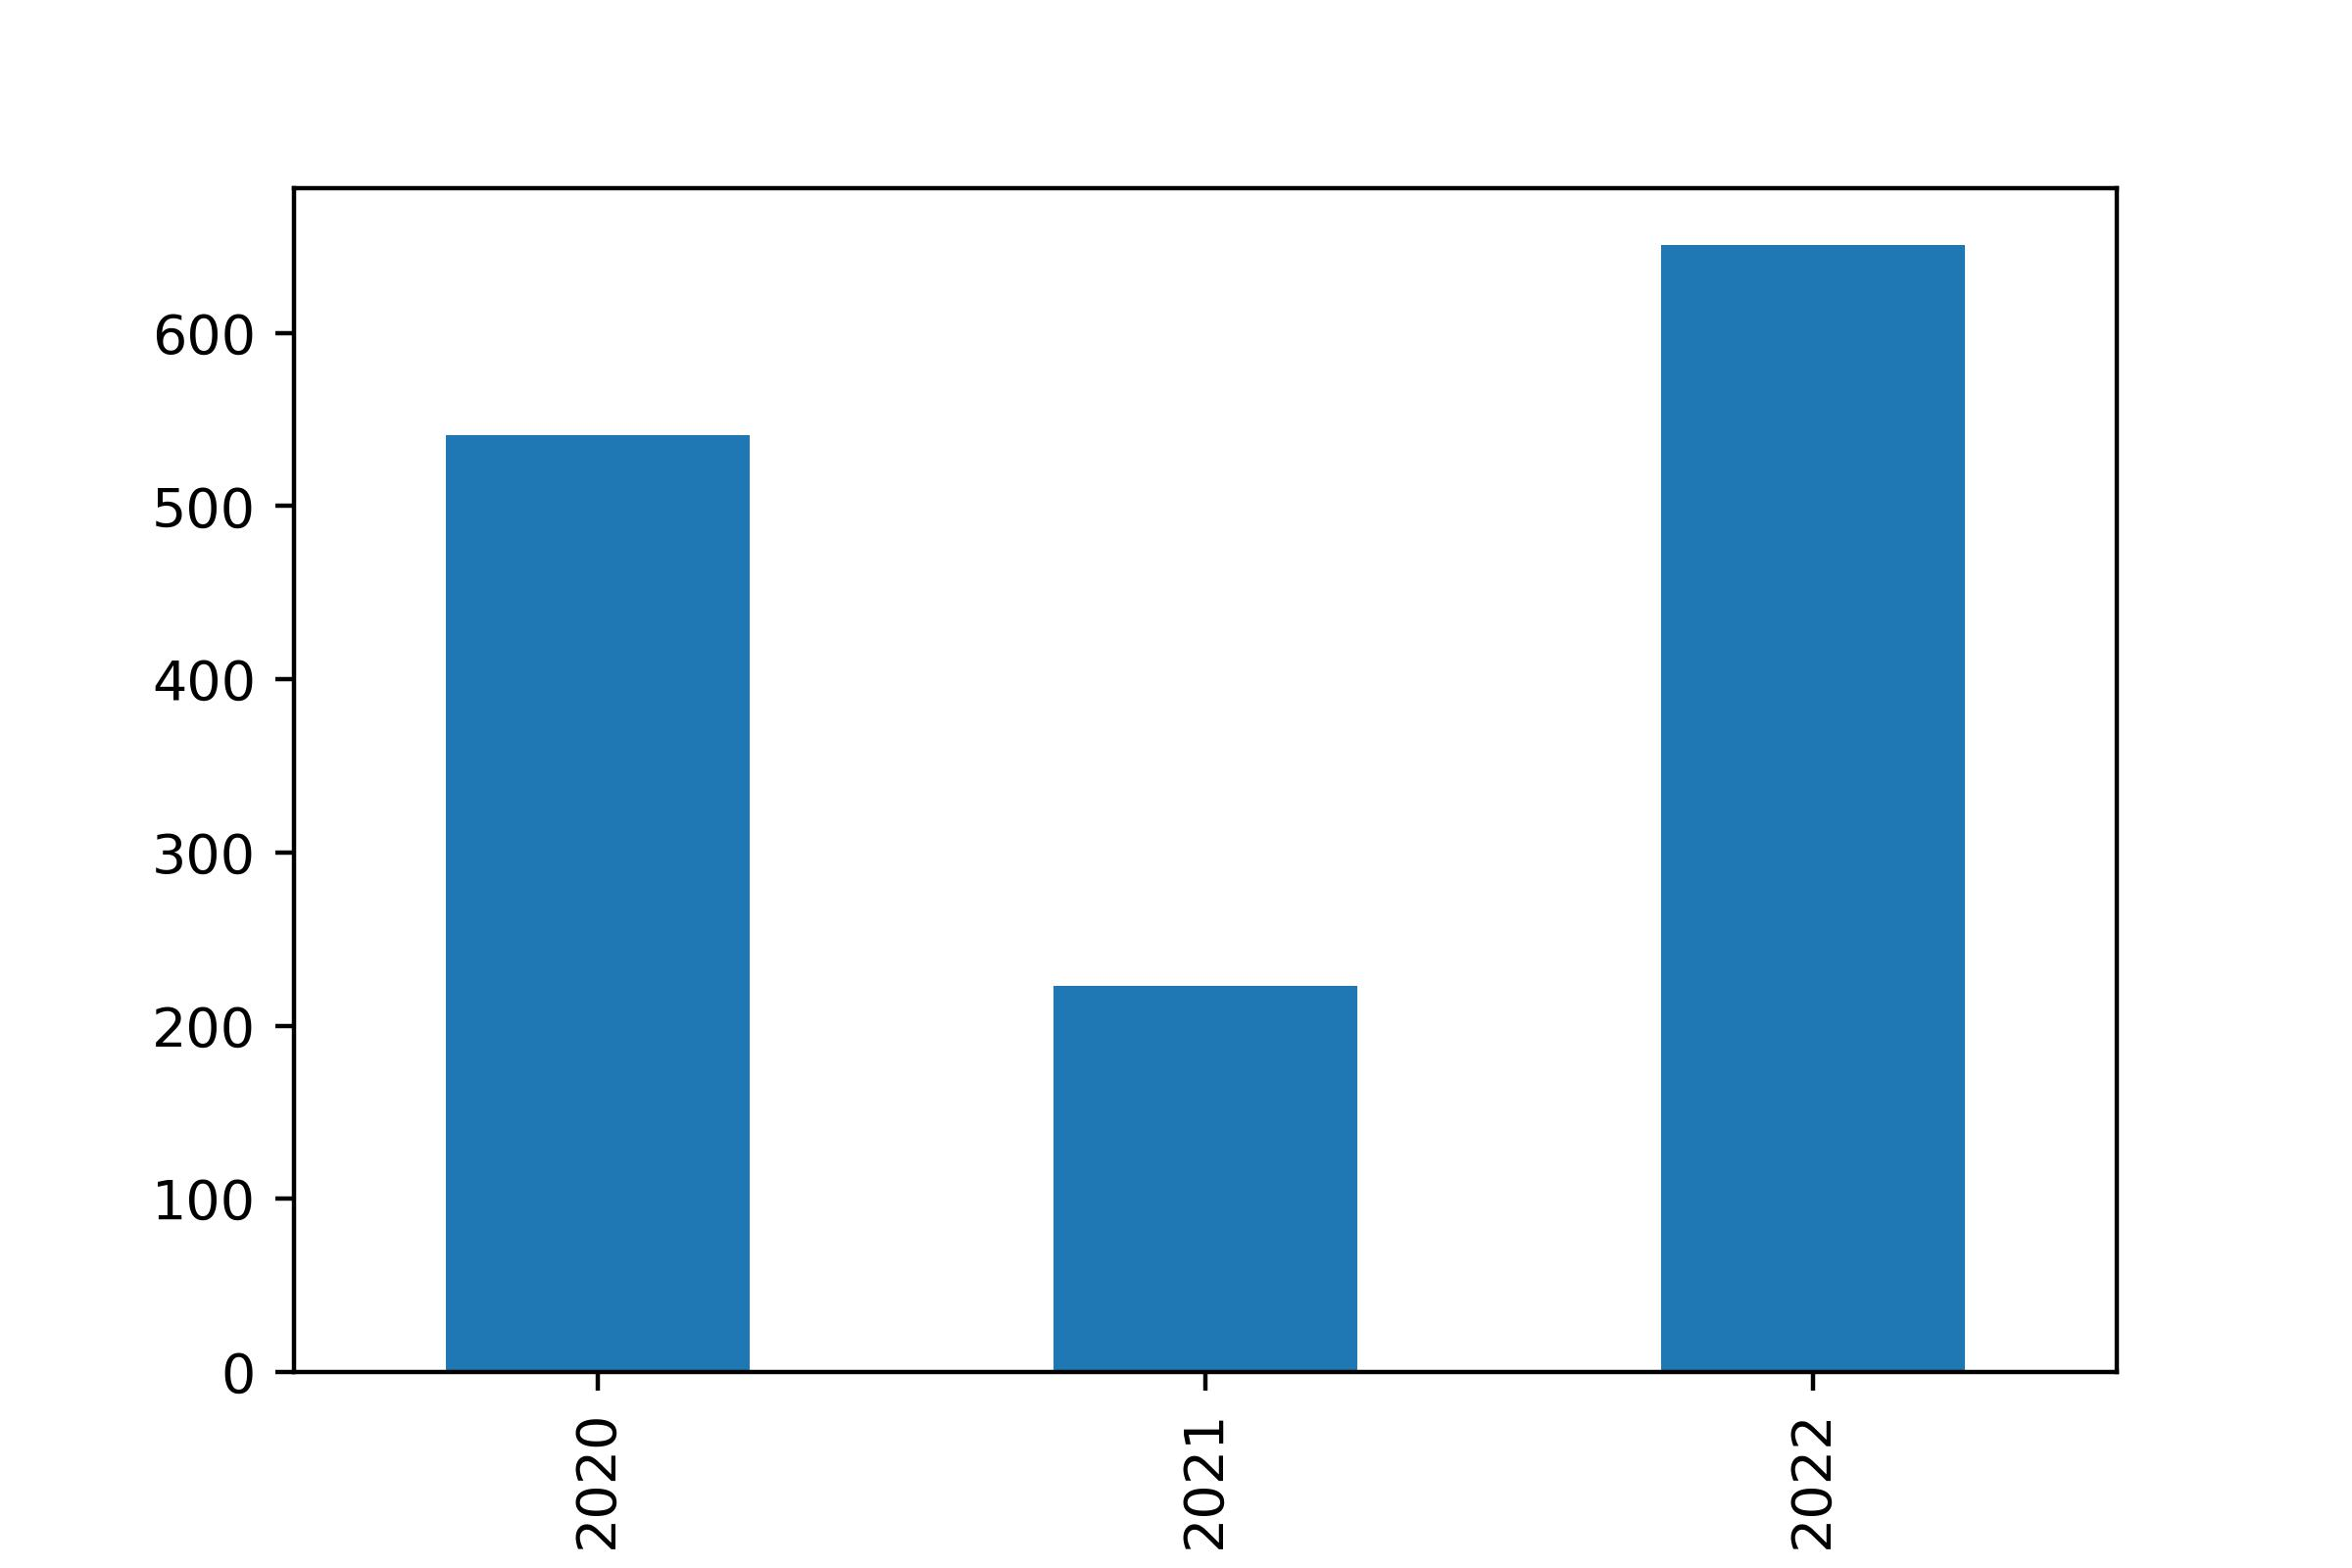
\includegraphics[width=\linewidth]{dist_merged.jpg}
\caption{Distribution of the full data set in time}
\label{fig:dist_merged}
\end{minipage}
\label{time_dist}
\end{figure}


I describe the composition of current product pages data as compared to the final data set in table \ref{table:decomp} in more detail. My original idea was to use the GitHub Issues logs to evaluate the rate of software development, however, the app pages that list a Google Play link rarely provide open source code, unless their developers are already highly respected in the community. The share of observations with both Google Play links and GitHub links restricts the sample too much, but I introduce the dummy for available GitHub page into the data set to control for different incentives driving the producers with open source code. 


As an alternative to this variable I collected comments for all product pages used in the analysis. There is a number of variables that I intend to use for estimation: first of all, it is the rate of developer messages to consumer messages, which should reflect how actively the developer is looking into the software bugs and issues that consumers report. Another variable, and the one I use for the first OLS regression, is the proportion of direct developer replies to messages in the product page. From the scraped data it is evident that the producers of actively developing products interact with their consumers a lot and address the problems that have been reported in each update. The summary statistics for the variables corresponding to forum page activities are shown in table \ref{table:cont}. I intend to add an additional variable, counting only the messages of consumers with words "bug", "doesn't work" and one with the number of direct developer replies divided by all comments in the thread. 


\begin{table}[!htbp] \centering 
\caption{Descriptive Statistics} 
  \label{table:decomp} 
    \begin{tabular}{|l|c|c|c|c|c|c|c|c|}
        \hline 
    \multirow{2}{*}{Filter}  & \multicolumn{3}{c|}{All Product Pages} & \multicolumn{3}{c|}{Estimation Sample}&\multicolumn{2}{c|}{Uncensored Sample} \\ 
        \cline{2-9} 
       & 2020 & 2021 & 2022 &2020&2021&2022&2020&2021\\ 
         \hline
    (1) contain ads  & - & - & - & 0.62 & 0.61 & 0.6& 0.63 & 0.625 \\ 

    (2) contain paid features  & - & - & - & 0.51 & 0.49 & 0.52 & 0.47 & 0.49 \\ 
    
    (3) both (1) \& (2)  & - & - & - & 0.34 & 0.33 & 0.35& 0.34 & 0.35 \\ 
    
    (4) contain a GitHub link  & - & - & 0.05 & 0.09 & 0.1 & 0.09 & 0.08 & 0.09\\ 
    
    (5) contain a Google Play link  & - & - & 0.4 & 1.00 & 1.00 & 1.00 & 1.00 & 1.00\\ 
    
    (6) both (4) \& (5)   & - & - & 0.02 & 0.09 & 0.1 & 0.09  & 0.08 & 0.09\\ 
    
    (8) mentioned in external threads  & WIP & WIP & WIP & 0.27 & 0.26 & 0.22 & 0.27 & 0.26 \\ 
    
    (9) positive response rate  & 0.04 & 0.03 & 0.03 & 0.22 & 0.2 & 0.09 & 0.16 & 0.13 \\
    
    (10) team of developers & - & - & 0.005 & 0.02 & 0.02 & 0.02 & 0.02 & 0.03\\
    
   
    \hline
    
    Share of obs. per year  & 0.31 & 0.155 & 0.535 & 0.38 & 0.16 & 0.46 & 0.73& 0.27 \\
    Obs. per year   &  7624& 3844&  13,191& 541 & 223 & 651 & 468 & 176 \\
        \hline 
    All obs.& \multicolumn{3}{c|}{ 24659 obs. (13191 unique firms)} & \multicolumn{3}{c|}{1415 obs. (671 firms)}&\multicolumn{2}{c|}{644 obs.} \\
    \hline
    \end{tabular} 
    \end{table} 
 
 
 
 
 
 
 
 
 
 
 
 
 
 
 
 
 
 
 
 
 
 
 
 
 
 
 
 
 
 
    \begin{table}
    \centering
       \caption{Descriptive Statistics of Developer Hierarchy ($w_x^j$)} 
  \label{table:title_decomp} 
  \begin{tabular}{|l|c|c|c|c|c|c|c|c|}
        \hline 
    \multirow{2}{*}{Filter}  & \multicolumn{3}{c|}{All Product Pages} & \multicolumn{3}{c|}{Estimation Sample}&\multicolumn{2}{c|}{Uncensored Sample} \\ 
        \cline{2-9} 
       & 2020 & 2021 & 2022 &2020&2021&2022&2020&2021\\ 
         \hline

    (4) (Senior) Recognized Developer   & 0.03 & 0.04 & 0.05 & 0.11 & 0.11 & 0.11 & 0.09 & 0.11\\ 
    
    (3) Senior Member & 0.35 & 0.4 & 0.42 & 0.62 & 0.59 & 0.59 & 0.62 & 0.59 \\ 
    
    (2) Member  & 0.16 & 0.34 & 0.33 & 0.26 & 0.27 & 0.28 & 0.28 & 0.28\\ 
    
    (1) New Member  & 0.03 & 0.07 & 0.13 & 0.01 & 0.02 & 1.00 & 0.01 & 0.02\\ 
    \hline
 
    Obs. per year   &  7624& 3844&  13,191& 541 & 223 & 651 & 468 & 176 \\
        \hline 
    All obs.& \multicolumn{3}{c|}{ 24659 obs.} & \multicolumn{3}{c|}{1415 obs.}&\multicolumn{2}{c|}{644 obs.} \\
    \hline
    \end{tabular} 
    \end{table} 




The demand, collected from Google Play, is represented as a step function, as the app only reports when the demand reaches above the certain level. I describe the distribution of demand values in table \ref{table:demand} and adjust this number in the estimation by using years since launch dummies. As the WayBack Machine collects timestamps from many different IPs, I am currently in the process of re-writing the scraper to adjust for languages other than English used in the page setup. As the IPs are random, the only way the measurement error may affect my results is by adding too much noise so that the parameters are insignificant. However, there seems to be an error in  collection of the dummy for paid apps, with a big fraction of false positive values. This is why for the preliminary analysis I am restricted to estimation of development rate and can not yet estimate the probability of offering aid good. The descriptive statistics of the data set by these variables is available in table \ref{table:decomp}.


 There is a number of options that developers have to monetize their product, on top of providing a free version at the forum. Table \ref{table:decomp} describes the share of monetized apps by their group in time. In the estimation I intend to use a number of possible interpretations of paid/not paid dummies ($Pr(p_{\tau}>0)$), both containing different monetized app groups and one with only completely paid apps and dummies for all other options.
 
    \begin{table}
    \centering
       \caption{Descriptive Statistics of Demand ($d_t$)} 
  \label{table:demand} 
  \begin{tabular}{|l|c|c|c|}
        \hline 
    Demand level & 2020 & 2021 & 2022 \\ 
       \hline
    1M+ & 0.37 & 0.34& 0.38\\
    
    1000+ - 500000+& 0.57 & 0.6 & 0.58\\ 
    
    1+ - 500+ & 0.05& 0.07 & 0.03\\ 
    \hline
   
    Obs. per year   &   541 & 223 & 651 \\
        \hline 
    All obs.& \multicolumn{3}{c|}{1415 obs.} \\
    \hline
    \end{tabular} 
    \end{table} 




As the data is so recent, there is a concern about censoring. I classify apps, which have not been updated in the last 6 months as ones at the end of their lifetime. This classification gives an approximate amount of 55 \% of censored data. I present the breakdown of both parts of the data set in table \ref{table:decomp}. As can be seen from this table, the composition between two fractions is not so dissimilar so as to cause concern.

For proxies for the wage costs I use a number of developer statistics, which are set by the forum. First of all, all developers have a title, which is a reflection of their hierarchy status in the forum. I describe the distribution of titles among the product developers in \ref{table:title_decomp}. In \ref{table:cont} I describe the continuous proxy variables that describe the developer. Developer messages correspond to the overall number of messages the developer posted on the forum. Due to huge variance of the variable it might be prudent to split it into a number of categorical variables instead, as there seems to be a huge gap between an average producer and some very active recognized contributors on the forum. At the same time, developer reactions corresponds to the inside-forum reputation system, where other members say thanks for useful contributions of the developers. There is another variable "developer points", which I intend to collect as another proxy. Lastly, I collect the size of developer team as an additional explanatory variable, although the variable does not change in time. I hope in the future to collect also the number of products that each developer is developing at the same time, but this is still work in progress.

   \begin{table}[t]
   \centering
       \caption{Description of Continuous Variables} 
  \label{table:cont} 
  \begin{tabular}{|c|l|c|c|c|c|}
\hline
                 &  & statistic &           2020 &          2021 &         2022 \\
\hline
 &response rate & mean &       0.135 &      0.098 &       0.026 \\
  &                 & std &       0.3 &      0.25 &     0.14 \\
 &                  & min &            0.0 &           0.0 &          0.0 \\
$\Delta s$    &               & max &            1.0 &           1.0 &          1.0 \\


 &developer replies & mean &    1.89 &    2.25 &   0.25 \\
&      & std &   20.18 &   21.89 &   3.48 \\
 &     & min &    0.00 &    0.00 &   0.00 \\
  &    & max &  449.00 &  306.00 &  83.00 \\



\hline
&developer reactions & mean &   27487.02 &  15918.16 &   2171.85 \\
 &                  & std &  141575.83 &  99513.54 &  11877.97 \\
  &                 & min &              0 &             0 &            0 \\
   $w_x$ &                & max &        1363970 &       1364240 &       136417 \\
&developer messages & mean &    9880.94 &   8268.61 &    886.09 \\
&                   & std &   29528.26 &   24552.16 &  2622.39 \\
&                   & min &             10 &             0 &            0 \\
&                   & max &         247250 &        247270 &        25652 \\
\hline
\multicolumn{2}{|l|}{Estimation Sample: } & \# obs &   541 & 223 & 651 \\
\hline
\end{tabular}
    \end{table} 



Lastly, I describe the variables that I use to measure $\gamma$, the probability of information sharing. Using the XDA Developers search engine I collected all external mentions of each product within the main forum, which appeared either as a mention in a thread of forum or in a specific post. Using this data, I created a dummy variable for mentions in external threads, which is described in table \ref{table:decomp}. Unfortunately, the results might be skewed for the apps with more general words used in the app title, as there can be mistaken search results in the collected data. To adjust for that, as well as possible competition between similar apps, I intend to add two correction variables: one, which evaluates the share of commonly used words in the app name, as well as one that reflects the share of words commonly used inside the forum. The descriptive statistics for these variables are also available in table \ref{table:cont}.

The main challenge I am facing still is collecting unique users in the sub-forums, where the external threads occur. The average number of these users will be my main proxy for $N$, as it reflects a fraction of how many people become informed on average through the information diffusion, as not all of them read all the posts in the sub-forum, and not all of those, who have read the mention, will leave a comment in kind. As the collection through search engine is much more time-consuming than other web-scraping procedures I used for the preliminary data, I am currently unable to provide statistics for all product pages with regards to these variables, as denoted in the table \ref{table:decomp} as "WIP".

\begin{table}

\caption{Rate of quality development and WOM}
\label{tab1}
\def\sym#1{\ifmmode^{#1}\else\(^{#1}\)\fi}
\begin{tabular}{l*{2}{c}}
\hline\hline
            &\multicolumn{1}{c}{(1)}&\multicolumn{1}{c}{(2)}\\
            &\multicolumn{1}{c}{Rate of dev. replies}&\multicolumn{1}{c}{Rate of dev. comments}\\
\hline
Demand category&     0.00803\sym{**} &     -0.0189\sym{**} \\
            &   (0.00348)         &   (0.00941)         \\
[1em]
Developer level in hierarchy    &      0.0111\sym{***}&      0.0257\sym{***}\\
            &   (0.00285)         &   (0.00772)         \\
[1em]
No change in demand category \& mentioned in external threads&      0.0124\sym{**} &      0.0158         \\
            &   (0.00566)         &    (0.0153)         \\
[1em]
Change in demand category \& no external threads mentions&    -0.00222         &     -0.0217         \\
            &   (0.00732)         &    (0.0198)         \\
[1em]
Change in demand category \& mentioned in external threads&      0.0153         &    -0.00351         \\
            &    (0.0125)         &    (0.0338)         \\
[1em]
No external threads mentions \& app name without frequently used words&     -0.0127\sym{**} &     -0.0297\sym{*}  \\
            &   (0.00635)         &    (0.0172)         \\
[1em]
No external threads mentions \& app name with frequently used words&   -0.000480         &    -0.00656         \\
            &   (0.00450)         &    (0.0122)         \\
[1em]
Product has a GitHub page       &      0.0133\sym{**} &      0.0186         \\
            &   (0.00637)         &    (0.0172)         \\
[1em]
Constant     &     -0.0358\sym{***}&      0.0541\sym{*}  \\
            &    (0.0115)         &    (0.0312)         \\
\hline
N           &        1401         &        1401         \\
Adjusted R-squared        &          0.1053           &            0.4168         \\
\hline\hline
\multicolumn{3}{l}{\footnotesize Standard errors in parentheses}\\
\multicolumn{3}{l}{\footnotesize \sym{*} \(p<0.1\), \sym{**} \(p<0.05\), \sym{***} \(p<0.01\)}\\
\end{tabular}

\end{table}

% \begin{table}[htbp]\centering
% \def\sym#1{\ifmmode^{#1}\else\(^{#1}\)\fi}
% \caption{Testing predictions of equation (2.1) \label{tab1}}
% \begin{tabular}{l*{1}{c}}
% \hline\hline
%             &\multicolumn{1}{c}{(1)}\\
%             &\multicolumn{1}{c}{Developer replies}\\
% \hline
% Demand category&       1.529\sym{*}  \\
%             &      (1.94)         \\
% [1em]
% Developer level in hierarchy    &       1.830\sym{***}\\
%             &      (3.11)         \\
% [1em]
% Product has a GitHub page    &       6.102\sym{***}\\
%             &      (4.22)         \\
% [1em]

% No change in demand category \& mentioned in external threads&       3.598\sym{***}\\
%             &      (2.81)         \\
% [1em]
% Change in demand category \& no external threads mentions&     -0.0259         \\
%             &     (-0.02)         \\
% [1em]
% Change in demand category \& mentioned in external threads&       3.839         \\
%             &      (1.35)         \\
% [1em]
% No external threads mentions \& app name with frequently used words&       0.228         \\
%             &      (0.22)         \\
% [1em]
% Mentioned in external threads \& app name with frequently used words&      -3.775\sym{***}\\
%             &     (-2.61)         \\
% [1em]
% Constant     &      -8.396\sym{***}\\
%             &     (-3.54)         \\
% \hline
% \(R^2\)       &        0.0429        \\
% \(N\)       &        1402         \\


% \hline\hline
% \multicolumn{2}{l}{\footnotesize \textit{t} statistics in parentheses}\\
% \multicolumn{2}{l}{\footnotesize \sym{*} \(p<0.10\), \sym{**} \(p<0.05\), \sym{***} \(p<0.01\)}\\
% \end{tabular}
% \end{table}

% \begin{table}[htbp]\centering

% \caption{Preliminary estimation of equation (2.4)}

% {
% \def\sym#1{\ifmmode^{#1}\else\(^{#1}\)\fi}
% \begin{tabular}{l*{4}{c}}
% \hline\hline
%             &\multicolumn{1}{c}{(1)}&\multicolumn{1}{c}{(2)}&\multicolumn{1}{c}{(3)}&\multicolumn{1}{c}{(4)}\\
%             &\multicolumn{1}{c}{Paid features in app}&\multicolumn{1}{c}{Paid features in app}&\multicolumn{1}{c}{Paid features in app}&\multicolumn{1}{c}{Paid version}\\
% \hline
% Developer reactions&0.000000296\sym{**}& 0.000000373\sym{*}& 0.000000358\sym{*}&   -8.32e-08       \\
%          &(0.000000142)       &(0.000000138)       &(0.000000138)       &  (7.90e-08)          \\
% [1em]
% Predicted $\Delta s$   &      0.0271\sym{*}&    -0.00102       &      0.0218       &      0.0144       \\
%   &   (0.00692)       &   (0.00729)       &    (0.0182)       &    (0.0104)       \\       \\
% [1em]
% Predicted $\Delta s^2$&    -0.00190\sym{*}&    0.000493       &     0.00120       &    0.000966       \\
%         &  (0.000989)       &  (0.000988)       &   (0.00112)       &  (0.000638)          \\
% [1em]
% Demand category&                   &       0.258\sym{*}&       0.275\sym{*}&     -0.0483\sym{*}\\
%           &                   &    (0.0264)       &    (0.0292)       &    (0.0167)              \\
% [1em]
% Demand category $\times$ predicted $\Delta$&                   &                   &     -0.0117       &    -0.00679       \\
%              &                   &                   &   (0.00852)       &   (0.00488)       \\
% [1em]
% Constant      &       0.489\sym{*}&      -0.102       &     -0.137\sym{**}&       0.601\sym{*}\\
%              &    (0.0148)       &    (0.0623)       &    (0.0672)       &    (0.0384)           \\
% \hline
% $R^2$  &            0.0289        &         0.0914       &           0.7028        &     0.7028                \\
% Within $R^2$&          0.0176     &           0.0809        &            0.6987       &      0.0150                \\
% N           &        1400       &        1400       &        1400       &        1400       \\
% \hline\hline
% \multicolumn{5}{l}{\footnotesize Standard errors in the parenthesis}\\
% \multicolumn{5}{l}{\footnotesize \sym{*} \(p<0.10\), \sym{**} \(p<0.05\), \sym{*} \(p<0.01\)}\\
% \end{tabular}
% }
% \end{table}

\begin{table}

\centering
\caption{Preliminary estimation of equation (2.5)}
\label{tab2}
\def\sym#1{\ifmmode^{#1}\else\(^{#1}\)\fi}
\begin{tabular}{l*{4}{c}}
\hline\hline
            &\multicolumn{1}{c}{(1)}&\multicolumn{1}{c}{(2)}&\multicolumn{1}{c}{(3)}&\multicolumn{1}{c}{(4)}\\
            &\multicolumn{1}{c}{Paid features}&\multicolumn{1}{c}{Paid features}&\multicolumn{1}{c}{Paid app}&\multicolumn{1}{c}{Paid app}\\
\hline
Developer reactions& 0.000000458         & 0.000000502         & 0.000000212         & 0.000000218         \\
            &(0.000000322)         &(0.000000322)         &(0.000000152)         &(0.000000152)         \\
[1em]
Lag of Demand      &       0.129         &       0.126         &    -0.00408         &    -0.00735         \\
            &    (0.0802)         &    (0.0804)         &    (0.0379)         &    (0.0379)         \\
[1em]
Demand category&       0.144\sym{*}  &       0.149\sym{*}  &     -0.0541         &     -0.0502         \\
            &    (0.0821)         &    (0.0823)         &    (0.0388)         &    (0.0388)         \\
[1em]
\# of developers &       0.109         &       0.106         &     -0.0517         &     -0.0514         \\
            &     (0.110)         &     (0.110)         &    (0.0521)         &    (0.0520)         \\
[1em]
Rate of replies ($\Delta s$)   &       0.628\sym{*}  &                     &       0.207         &                     \\
            &     (0.364)         &                     &     (0.172)         &                     \\
[1em]
Rate of comments($\Delta s$) &                     &      0.0552         &                     &       0.125\sym{**} \\
            &                     &     (0.125)         &                     &    (0.0590)         \\
[1em]
Constant      &      -0.230         &      -0.230         &       0.327\sym{***}&       0.323\sym{***}\\
            &     (0.142)         &     (0.142)         &    (0.0671)         &    (0.0670)         \\
\hline
N           &         736         &         736         &         736         &         736         \\
Adjusted R-squared         &            0.0864          &            0.0829         &        0.5766              &          0.5784           \\
\hline\hline
\multicolumn{5}{l}{\footnotesize Standard errors in parentheses}\\
\multicolumn{5}{l}{\footnotesize \sym{*} \(p<0.1\), \sym{**} \(p<0.05\), \sym{***} \(p<0.01\)}\\
\end{tabular}
\end{table}


\textbf{Preliminary results and discussion:}

While I am still missing the proxy for $N$ and instruments for demand, I can test some model predictions via OLS in order to check whether the effects the model predicts are there. Using the variables in equation (2.3), I first estimate a simple OLS of the form:

$$\Delta s_{it} = a_0 + a_1M_{it} + a_2w_{it} + a_3I_{M_{it} -  M_{it-1}>0} \times I_{\gamma_{it}>0} + a_4I_{\Delta M_{it-1}>0}\times D_{corr} + \mu_{it}$$

where $D_{corr}$ corresponds to a dummy I include for correction of measurement error from $\gamma_{it}$ collection. I also include interaction terms to see if the effects of the variables vary between different subsets of observations, and a dummy for available GitHub page, careful of considerations described above. In line with the predictions of the model, all variables have significant coefficients.  The results of the estimation are available in the table \ref{tab1}.

Especially interesting are the coefficients for the interaction terms. As the model predicts, mentions in external threads affect positively the development of the good even if the demand category does not change between periods. This supports the argument that WOM communication influences the product development. Similarly, if there was a change in demand, then the development is higher, if there are external mentions of the product in the forum (significant on 85\% level, which can be due to a very likely measurement error in the variable), which means that there is not only the effect of new consumers becoming aware of the good, but also an additional effect of them diffusing information. It must be said, however, that the results need to be taken with a grain of salt, as I do not account for the endogeneity bias from regressing quality development on demand, which depends on price, yet. My suggestions for the possible demand instruments can be found in the Empirical strategy subsection.

The dummy for fraction of frequently used words in the app name not only helps correct for the false positive results of the search engine, but also hint that there might be similar apps on the markets, and they reduce the effect of the external mentions. I plan to investigate the issue further and try to exclude markets with more than one innovator from the final data set.

Intuitively, developers who make their GitHub page available to other producers are more likely to invest in developing quality via interaction in the forum. I am planning to include this variable as a control also in the final estimation, as my expectation would be that these consumers derive higher benefit from feedback.

Secondly, I estimate a number of preliminary OLS regressions for equation (2.5), the results of which are showed in table \ref{tab2}. The results of this regression also need to be taken with a grain of salt, as the endogenity concern is completely ignored here. The regression has the following form:

$$I_{p_{it}>0} = b_0 + b_1w_{it} + b_2M_{it-1} + b_3M_{it} + b_4\Delta s_{it} + \nu_{it}$$

The inclusion of the lagged demand here is necessary, as per model assumptions it is through accumulated demand that the consumer feedback affects the probability of offering a paid version of the good. It restricts the estimation sample to 740 observations; however, the coefficient before lagged demand is positive and significant on 85\% level for model 1 and 2, despite the inclusion of the current demand into the estimation, which shows promise. Both variables for software development rate are significant in different specifications of the model, which supports the model specification.


To conclude, the testing predictions of the first half of the model with OLS, I find the expected positive relationship between software development and WOM communication, as well as lagged demand and probability of entry, which corresponds to the effect of consumer feedback. Despite possible concerns about endogeneity, I expect to provide additional evidence to support these arguments in the future estimations, once I have collected all of the variables.

%\section{Conclusion}
\newpage
\section{Dynamic Model of Innovative Quality in Markets with WOM Communication}

While in the second section of the research proposal I address the possible ramifications of WOM communication in the quality development decision of the incumbent in a platform, where she is forced to always provide a freely available good, in this project I investigate in more detail the incentives of the incumbent to participate in such a platform. The main research question I intend to answer with this project is: when is it optimal for an innovative incumbent to provide a free good and what role WOM communication plays in this decision? I aim to examine, what is the optimal quality development and pricing policy of an incumbent in a market with copying and WOM effects, and how these factors determine the lifetime and survival of a product.

Introducing a more complex information exchange between consumers, I now assume that it is not the information about the good's existence that is being diffused, but instead about its quality. However, there is an element still of delayed information diffusion: while consumers communicate quality to each other, they only do it after they have themselves tried the good. In this setup the incumbent is additionally incentivized to attract consumers so as to promote information diffusion.

On top of the already mentioned literature on WOM and differentiated goods, this project draws on the extensive good reputation literature. Similar to \citet{Board2014}, I look into the market beliefs about the quality of the good as the consumers are unsure about the good's quality. In my project, however, the uncertainty about quality only exists until the good is tried, as it is less an issue of reputation and more an issue of asymmetry of information. My goal is not to investigate the reputation dynamics, but rather the quality dynamics and the information-based incentives that the incumbent has to continue developing her good. 

Methodologically, if not thematically, I rely on \citet{Isaac2003}, who investigates the survival of the good, where its reputation is updated according to Bayes' rule. While I also am interested in the good's survival and its dependence on the information diffusion, my main contribution is that the quality of the good is not set, but developed in an optimal way. In fact, this comparative ease of quality updates is characteristic of digital goods markets, which are, as rule, either updated regularly or abandoned.

In light of this developing a model, which explains such a dynamic seems prudent. In the following sections I set up the baseline and the extended models and explain both preliminary and expected results. I clarify how these results correspond to the assumptions I set in the empirical model in section 2 and extrapolate on what additional insights can be gained from this project. 


\subsection{Fundamentals of the Baseline Model}
In the following subsection I set up the dynamic model of quality development. The game continues as long as the expected profit of the incumbent is non-negative. Once the the innovative producer perceives that she can not gain profit from participating in the market, she exits the market.

\textbf{Supply:}
Consider a market with two producers: incumbent and entrant. The incumbent enters the market with an innovative idea in $t=0$. The entrant, who is only capable of copying the incumbent's good, enters one period later. The goods on the market are vertically differentiated, and producing new quality is costly. Once produced, the quality can be copied perfectly with a delay of one period. The incumbent starts with some initial quality of the good, which I normalize to 0, and in each period may invest some $c$ to update the quality of the good by the same increment $\Delta s$. The cost of quality development is independent of sold quantity, as the consumers pay $p_t^{inc}$ as a subscription price for accessing the good. The price that the incumbent sets is constrained at 0.

\textbf{Demand:} Consumers value quality, but initially are not informed about its real value. They form beliefs about the producer's ability to produce quality, so that each quality increment is discounted by $\lambda$: $E(\Delta s) = \lambda \Delta s$. In the baseline model I assume that $\lambda$ only takes two values: $0\leq\lambda_0 <1$ in the initial period and $\lambda=1$ for all quality increments that the consumer has experienced or experienced second-hand through their friends. Following \citet{Tirole},  $u_j = \lambda \theta_j s_t - p_{ti}$, where $i$ is either an incumbent or an entrant and $\theta$ - is drawn separately and independently from $U[0,1]$ every period and signifies the taste for quality of consumer $j$. This assumption serves to deter the incumbent from learning about her consumers with each period. All consumers have an outside option, the value of which is 0. Each consumer only needs one good of a certain quality, and may only pay for additional quality, if it is offered.

\textbf{Timing:} 
In $t=0$ incumbent enters the market and chooses: (1) whether to develop quality above 0, resulting in $s_0$, (2) what price $p_0^{inc}$ to offer for the good, (3) whether to participate in the trade, depending on her expected profit from these optimal quality and price. In $t=0$ the market only consists of M consumers, who are sceptical about the good's quality. They perceive the incumbent's decision to develop, but if she does, they only perceive the quality as $\lambda_0 \Delta s$. They observe the pricing and decide whether to purchase. If they do, they realise the good's quality and are now aware of its true value.

In $t=1$ all consumers who have purchased the incumbent's good inform $N$ of their friends about it, resulting in incumbent's customer base expansion by $d_0N$ consumers, where $d_0$ is the realised demand in the period zero. An entrant then copies the good of the incumbent in the previous period and decides on (1) what price $p_1^{e}$ to offer for the good of quality $s_0$, (2) whether to participate in the trade, based on her expected profits. She can only reach the original customer base of $M$ consumers, $d_1$ of which are already informed about the incumbent's previous period good's quality. These $M$ consumers do not know that she is copying the incumbent's good and thus are expecting her quality to be also only as $\lambda_0 s_0$. The incumbent, simultaneously with the entrant, decides (1) whether to develop the good further, (2) what price $p_1^{inc}$ to offer for the new good, and (3) whether to continue trading. 

The interaction in $t=1$ repeats until the incumbent decides to stop participating in the market and abandons her product. 

\subsection{Expected Results, Conjectures and Future Work} 
 The maximisation problem of the incumbent in period 0, where $max\{V(0, V(\textbf{p}, \textbf{s})\}$ corresponds to the expected profit of the incumbent, when she follows an optimal pricing $\textbf{p}$ and development strategy $\textbf{s}$. 
$$
\begin{aligned}
\max_{p_0,s_0} \quad &  M(1-\tfrac{p_0^{inc}}{\Delta s})p_0^{inc} - c + \beta \max\{0, V(\textbf{p}, \textbf{s})\}\\
\textrm{s.t.} \quad &p_0 \geq 0\\
\end{aligned}
$$

If the producer is completely myopic, her optimal price, if she decides to develop quality, in the zero period is $p_0=\tfrac{\lambda_0 \Delta s }{2}$. In light of this, the incumbent only decides to develop quality if the consumers are not to sceptic about the good; in the myopic case, $\lambda_0 \geq \tfrac{4c}{M\Delta s}$. I anticipate that this threshold can be reduced to 0 through the expectation of future profit, and the incumbent might find it optimal to produce quality and offer this good for free to outpace the entrant, when consumers are close to perfectly sceptic about the quality of the good for a number of periods.

\begin{conjecture}
There exists such $\tilde{t}$, $\hat{t}$ that for any period $t$, s.t. $\tilde{t} \leq t \leq \hat{t}$ it is optimal for the incumbent to set a non-zero price for her good. %If the incumbent finds it optimal to set a non-zero price for the good in period $\tilde{t}$, she will not deviate from the non-zero price strategy in any period $\tilde{t}\leq t \leq \hat{t}-1$, where $\hat{t}$ is the period when it is no longer optimal for her to develop quality. In period $\hat{t}$ she is forced to set the price to 0 and can not gain a positive profit in any period $t\geq \hat{t}$.
\end{conjecture}

In fact, her ability to set such a price is what incetivizes her to participate in the market. As the consumer base grows, she has less incentives to set the price equal to 0. As a conjecture, I anticipate that her optimal pricing strategy, depending on the prior belief $\lambda_0$ and $c$ will consist of first a number of periods with zero-pricing, then non-zero pricing until such a $\hat{t}$ where she can no longer attract consumers and exits the market.

%The intuition behind this result is as follows: by backwards induction, I start with the period $\hat{t}$. A period like that occurs if in period $t_{\hat-1}$ the incumbent faced 0 demand, and her delayed information diffusion advantage is lost, as everybody on the market has bought the entrant's good and is sure of its quality, which is the quality the incumbent has been producing up to period $\hat{t}-1$. As her good was not bought, her last period's developed quality is  suppose in period \underline{t} the incumbent prefers to set a non-zero price and participate in the trade. As the consumer only participates in the trade if she expects positive profit from it, it must be that 


Denoting the probability of each specific consumer consuming the good in period $\tau$ as $d_{\tau}$, assuming $t<20$ and using the conjecture that the incumbent will develop quality in any period she can set a non-zero price, I can express $\pi_t$, the profit in each period $\tilde{t} \leq t \leq \hat{t}$ through Poisson binomial distribution function and solve for the optimal pricing and development strategy. 

%$$\pi_t = M(\Pi^t_{\tau=0}(1-d_{\tau})(1-\tfrac{p_{t}^{inc}-p_t^{e}}{})$$

%The first term corresponds to the fraction of consumers who have never tried the incumbent's good. Assuming that the entrant sets the price so as to satisfy the participation constraint, they must have tried the entrant's good and are now aware of her previous period's quality. In their eyes the quality of the entrant can now be above the quality of the incumbent, as they have experienced the $t-1$ 


\textbf{Extension: Bayesian updating}

As an extension to the baseline model I would like to look into the possibility of Bayesian updating of consumer beliefs. The parameter $\lambda$ should now take more than two values, depending on what consumers observe of the behaviour of others.  I assume now that instead of directly talking about it, the consumers observe each others feedback and update their beliefs based on the posterior distribution of consumer benefits. To accommodate this setup I need to update the description of demand.

All consumers, who have tried the good, can now leave feedback for the producer about their benefit, that other consumers observe. Using the distribution of consumer benefits, the likelihood of the producer's quality being what she states, is updated. 

This setup allows me to infer information about a number of markets, where feedback and reviews play a role. This extension's main contribution is to investigate the dynamic of the information diffusion, where consumers take time to update their beliefs instead if immediately trusting other consumers.

\textbf{Extension: Menu of goods}

Finally, I would be especially interested into expanding this model to accommodate the ability of the incumbent to offer more than one good at the time and the question of whether and if it is optimal. "Freemium" pricing, demo versions of the goods and freely available software: providing a free version of the good is extremely common even among successful software companies. Expanding the project in this way I expect to find that this strategy is optimal to an incumbent who is forced to develop continuously and price lowly to keep the consumers in the dark about the entrant's offer and preserve her market advantage.

\newpage

\section{Penetration Pricing in Markets with Bargain-Hunting Consumers}

As my third project I would like to investigate the impact of consumer behaviour on entry in markets with pronounced WOM communication. In particular, I am interested in the propensity of consumers towards bargain-hunting and its influence on the success of such an entry strategy as penetration pricing. To my knowledge, this is a first project attempting to do such using expectations-based reference paradigm, as opposed to more classical demand estimation approaches in marketing literature \citet{penetration}.

I would like to explore the expectations-based price references effects, where consumers react more strongly to perceived gains from getting a bargain, than to perceived losses, in the context of its influence on the WOM communication intensity and thus, market entry. My research question for this project is: does bargain-hunting behaviour increase the probability of successful entry? 

This idea contributes to the rich literature pertaining to dynamic demand models empirical estimation, growing from the classic discrete choice models, such as \citet{BLP}, optimal pricing in markets with strategic consumers \citet{Lobel2016} and models of reference-dependent preferences \citet{Gentry2018}. My proposed project not only combines these branches, but builds upon them in a logical manner. 
While \citet{Gentry2021} explore the pricing decisions in markets with bargain-hunting consumers, their contribution is mainly theoretical and applicable to retail markets, which are more easily explained and estimated by discrete choice models and thus, have been explored extensively in literature. Less attention, however, has been paid to digital goods, the demand for which is often different in structure to classic models \citet{penetration}, and even less has been paid to the reference-based preferences in such a setting. My focus and application for the demand model are computer games, in particular, which makes the project additionally interesting.

My goal is to develop a dynamic demand model with reference effects in a market with an entrant, whose goal is to build a customer base among many competitive offers. The real world example, and also a prospective data set that I hope to use for such an estimation, would be a video game platform gog.com, which sells licensed online versions of video games for PC. The demand in such a market differs greatly from classical models. All consumers choose from a number of options, often purchasing multiple items within computer game categories. The consumer only purchases each game once, and can use it in perpetuity; however, the value of the game depreciates in time, and the pricing decisions of the producers will depend on the dynamic optimisation of the consumer, similar to the dynamic described by \citet{Gowrisankaran2012}. Implementing a similar model of dynamic demand, I would like to integrate the price-expectation paradigm into it and investigate how this would change the optimal behaviour of the consumer. My expectation would be that bargain-hunting consumers would be more likely to purchase goods during discounts, comparing their prices to prices of other products on the market than await the lowering of the price with time. From this, the next step would be to investigate the pricing decisions of the producers, who are aware of the allure of a bargain for consumers, and predict the optimal pricing strategy. Using the results from the structural model estimation I would like to look into the entry decision and entry strategy of a new producer or a new product, as a counterfactual.

The data that I hope to collect through web-scraping is rich enough to accommodate the estimation of such a model. The platform combines a store, where all games available for purchase are listed with their prices and characteristics, i.e. their compatibility with hardware; profile pages for all users, including information on the games they have purchased, the amount of hours played and their achievements in the games they are playing; and a forum, where players can discuss different games. 

My expectation from this estimation would be that the markets, where  there is a tendency towards bargain-hunting behavior, additionally incentivize producers to engage in penetration pricing to attract new consumers. 

\newpage
\bibliography{bibliography}

\end{document}
